\documentclass[12pt]{article}
\usepackage{graphicx}
\usepackage{amsmath}
\usepackage{amssymb}

\usepackage{lipsum}
\usepackage{listings}
\usepackage{hyperref}
\usepackage{siunitx}
\usepackage[citestyle=numeric, sorting=none, doi=false,isbn=false, url=false, eprint=false]{biblatex}
%\addbibresource{bibliography.bib}
\bibliography{refs}


\usepackage{xcolor}
\usepackage[british]{babel}
\usepackage{csquotes}
\addto\extrasbritish{\def\equationautorefname{Eq.}} % Autoref-name for equations
\addto\extrasbritish{\def\figureautorefname{Fig.}}  % Autoref-name for figures
\addto\extrasbritish{\def\tableautorefname{Table}}    % Autoref-name for tables
\addto\extrasbritish{\def\sectionautorefname{Section}}    % Autoref-name for sections
\addto\extrasbritish{\def\subsectionautorefname{\sectionautorefname}} % Autoref-name for subsections
\addto\extrasbritish{\def\subsubsectionautorefname{\sectionautorefname}} % 
 
\definecolor{codegreen}{rgb}{0,0.6,0}
\definecolor{codegray}{rgb}{0.5,0.5,0.5}
\definecolor{codepurple}{rgb}{0.58,0,0.82}
\definecolor{backcolour}{rgb}{0.95,0.95,0.92}
 
\lstdefinestyle{mystyle}{
    language=Python,
    backgroundcolor=\color{backcolour},   
    commentstyle=\color{codegreen},
    keywordstyle=\color{magenta},
    numberstyle=\tiny\color{codegray},
    stringstyle=\color{codepurple},
    basicstyle=\footnotesize,
    breakatwhitespace=false,         
    breaklines=true,                 
    captionpos=b,                    
    keepspaces=true,                 
    numbers=left,                    
    numbersep=5pt,                  
    showspaces=false,                
    showstringspaces=false,
    showtabs=false,                  
    tabsize=2
}
\lstset{style=mystyle}

\title{FYS-STK4155 - Project 2}
\author{Magnus Kristoffersen, Markus Bjørklund}
\date{November 2023}


\begin{document}

\maketitle

\begin{abstract}
We compared the effects of applying classical regression methods against using feedforward neural networks for solving regression and classification problems. The data set used to perform regression was sampled from a second order polynomial with a noise term, while the Wisconsin breast cancer data set was used to classify tumors as malignant or benign. The classical methods used to solve the regression problem were ordinary least squares and Ridge regression, and the classification problem was solved with logistic regression. Both the classical regression models and the neural network models were trained using plain and stochastic gradient descent methods, and using the adaptive optimization methods AdaGrad, RMSProp and ADAM. These solvers were studied for different values of the learning rate and regularization parameters. In addition, the neural networks were also studied with different activation functions in the hidden layers. The drawback of classical methods is that they are unable to find non-linear relations in complex problems, but for the data sets considered in this report, classical methods were able to achieve approximately the same accuracy as the neural networks. For the classification of the cancer data, the logistic regression with well tuned learning rate and regularization parameters was able to achieve accuracies in the range \numrange[range-phrase = --]{95.61}{98.25} \% on the test set, while the neural network was able to achieve \numrange[range-phrase = --]{97.37}{99.12} \%.

    
Code, figures and documentation can be viewed on GitHub\footnote{\url{https://github.com/marbjo/FYS-STK4155/tree/master/project2}}.
\end{abstract}

\section{Introduction}
Artifical neural networks (ANN), or simply neural networks (NN), are a class of machine learning methods which have proved themselves as a versatile and robust tool in modern-day machine learning. Loosely inspired by the brain, many different tasks such as image recognition, speech recognition and natural language processing \cite{Nielsen}, whether it be continuous (regression) or discrete (classification).
In this work, we will study neural networks by comparing them to regression methods, both linear regression and logistic regression. For the continuous case, we will fit a second order polynomial using both a neural network and classic linear regression. For classification, we will look at the Wisconsin Breast Cancer data set\cite{breast_cancer_wisconsin}, applying both the neural network and logistic regression.

\autoref{sec:theory} presents the theory of the linear and logistic regression models and for the neural network. The method is then described in \autoref{sec:method}. We present our results in \autoref{sec:results}, and these results are discussed further in \autoref{sec:discussion}. Finally, we provide our concluding remarks in \autoref{sec:conclusion}. Unless otherwise specified, the theory presented is gathered from the lecture notes in FYS-STK4155 \cite{lecture-notes}. 

\section{Theory} \label{sec:theory}

\subsection{Gradient descent}
For the regression problems that were solved in project 1 \cite{project1-report}, the solutions were determined analytically by performing matrix inversions to minimize the chosen cost function. For regression problems with higher numbers of features (columns in our design matrix), these matrix inversions become computationally expensive. For this reason, we have to instead use a method for approximating the minimum of a cost function. A set of popular choices of methods for performing this task is the family of gradient descent methods. The idea of these methods is to determine the minimum of a function iteratively by using that the value of a function $f(\boldsymbol{x})$ in a given point $\boldsymbol{x} = (x_1, \hdots, x_n)$ decreases fastest in the direction of the negative gradient of the function. This can be formalized by the iteration process
\begin{equation}\label{eq:grad_descent}
    \boldsymbol{x}_{(k+1)} = \boldsymbol{x}_{(k)} - \eta_{(k)} \nabla f\left( \boldsymbol{x}_{(k)} \right),
\end{equation}
where $\eta_{(k)}$ is the step length, often called the learning rate, used to update the position in each iteration. In the next section, we will present different models for the time (iteration number) dependence of the learning rate.

In our regression models, the goal is to find the regression parameters $\boldsymbol{\beta}$ that minimize the cost function. By using mean squared error as cost function, the cost function reads
\begin{equation}\label{eq:mse_plain}
    C(\boldsymbol{X}, \boldsymbol{y}, \boldsymbol{\beta}) = \frac{1}{n} ||\boldsymbol{y} - \boldsymbol{X} \boldsymbol{\beta} ||_2^2 = \frac{1}{n} \sum_{i=1}^n (y_i - \boldsymbol{X}_{i,*} \boldsymbol{\beta})^2,
\end{equation}
where $\boldsymbol{X}$ is the design matrix generated from the input data, $\boldsymbol{y}$ is the correct output and $n$ is the sample size. The gradient of the cost function with respect to the regression parameters is
\begin{equation}
    \nabla_{\boldsymbol{\beta}} C (\boldsymbol{\beta}) = - \frac{2}{n} \boldsymbol{X}^T \left( \boldsymbol{y} - \boldsymbol{X} \boldsymbol{\beta} \right).
\end{equation}

By replacing $\boldsymbol{x}$ and $f(\boldsymbol{x})$ with $\boldsymbol{\beta}$ and $C(\boldsymbol{\beta})$, respectively, in \autoref{eq:grad_descent}, we have an iterative method for approximating the regression parameters that minimize of the cost function. However, the method might converge to a local minimum, and not the global minimum of the cost function.

The method denoted as plain gradient descent calculates the gradients for an entire data set, and then updates the parameters. This method makes each step of the process dependent on all the entries in the data set, giving the actual gradient of the data set for the given $\boldsymbol{\beta}$ values. However, calculating the gradient of the entire data set in each iteration step becomes very computationally expensive for large data sets. 

The method known as stochastic gradient descent (minibatch gradient descent) attempts to reduce the computational cost of the minimization process by dividing the data set into minibatches of a specified number of data samples. For this method, the update of $\boldsymbol{\beta}$ in each iteration is only determined by the gradients of the data samples in a randomly drawn minibatch, decreasing the computational cost associated with calculating gradients significantly. Due to the stochasticity of this method, it may also make the process less likely to become stuck in a local minimum. 

A quantity known as momentum or memory is often introduced into gradient descent methods to improve both their ability to reach the global minimum and their efficiency (number of iterations before achieving convergence). The addition of momentum is represented by adding a term containing the change of $\boldsymbol{\beta}$ in the previous iteration multiplied with a tunable momentum parameter $\gamma_{(k)}$. By inserting the momentum term into \autoref{eq:grad_descent}, we obtain the expression
\begin{equation}\label{eq:grad_descent_momentum}
    \boldsymbol{\beta}_{(k+1)} = \boldsymbol{\beta}_{(k)} + \eta_{(k)} \nabla_{\boldsymbol{\beta}} C(\boldsymbol{\beta}) - \gamma_{(k)} (\boldsymbol{\beta}_{(k)} - \boldsymbol{\beta}_{(k-1)}).
\end{equation}

\subsection{Learning rate} \label{sec:learning_rate}
One of the hyperparameters defined in the gradient descent methods mentioned above is the learning rate. This parameter is related to the magnitude of change in the $\boldsymbol{\beta}$ parameters during one iteration. The simplest method is to choose a fixed value for the learning rate throughout the gradient descent process. 

The problem associated with using a fixed learning rate is that the gradient descent method may perform too large parameter updates when approaching a minima, making the method unable to achieve convergence by overshooting the minima. By using a learning rate with time decay, the updates of the $\boldsymbol{\beta}$ parameters will decrease as a function of the number of iterations, which will make the gradient descent method able to converge to the minima. This time decay method for the learning rate is often chosen as
\begin{equation} \label{eq:time_decay}
    \eta_{(t)} = \frac{t_0}{t + t_1},
\end{equation}
where $t$ is the number of iterations performed of the gradient descent, while $t_0$ and $t_1$ are tunable hyperparameters. The issue now is that we defined two new hyperparameters that need to be tuned. If the time decay of the learning rate is too large, the gradient descent will be unable to reach a minima because the updates of $\boldsymbol{\beta}$ will become negligible while the value of the gradient is still significant.

To circumvent issues associated with choosing the decay rate for the learning rate, several methods have been developed for making the learning rate adaptive to the curvature of the cost function landscape. These methods aim to have a small learning rate for steep gradients and a larger learning rate for flat gradients, such that the total change, or step, gets neither too small or too large. In order to determine the curvature of the landscape in the current position, these methods track the first and second moment of the gradient during the iterations. The adaptive methods we will consider is AdaGrad, Root Mean Squared Propagation (RMSProp) and ADAM.

The update scheme for AdaGrad is given as
\begin{equation}
    \boldsymbol{\beta}_{(k+1)} = \boldsymbol{\beta}_{(k)} - \eta \frac{\boldsymbol{g}_{(k)}}{\sqrt{(\boldsymbol{s}_{(k)})} + \delta},
\end{equation}
where $\boldsymbol{g}_{(k)} = \nabla_{\boldsymbol{\beta}_{(k)}} C(\boldsymbol{\beta})$ is the gradient of the cost function in the position in iteration $k$, and $\boldsymbol{s}_{(k)} = \sum_{i=0}^k \boldsymbol{g}_{(i)}^2$ is the accumulated second moment of the gradient during all the previous iterations. $\delta$ is a small constant to prevent the algorithm from dividing by zero.

The expression for the root mean squared propagation (RMSProp) looks similar to the expression for AdaGrad, except that the expression for the second moment is given as
\begin{equation}\label{eq:second_moment}
    \boldsymbol{s}_{(k)} = \rho_2 \boldsymbol{s}_{(k-1)} + (1 - \rho_2) \boldsymbol{g}_{(k)}^2,
\end{equation}
where $\rho_2$ is a hyperparameter deciding the weighting of the previous memory against the current second moment. 
By looking at this expression, we can notice that when the gradients are large over several iterations, the step length will be small, while if the gradients are mostly flat, the step length will be longer.

The final adaptive learning rate optimizer we will consider is ADAM. This method uses a running average of the second moment of the gradients, given in \autoref{eq:second_moment}, and the first moment of the gradients
\begin{equation}
    \boldsymbol{m}_{(k)} =  \rho_1 \boldsymbol{m}_{(k-1)} + (1 - \rho_1) \boldsymbol{g}_{(k)},
\end{equation}
where $\rho_1$ is a hyperparameter for the weighting between the previous memory and the current first moment of the gradient.
ADAM contains an additional bias correction for accounting for the first and second moment being estimated from the running averages. The update scheme for this method is given as
\begin{equation}
    \boldsymbol{\beta}_{(k+1)} = \boldsymbol{\beta}_{(k)} - \eta \frac{\boldsymbol{m}_{(k)} / (1 - \rho_1^k)}{\sqrt{\boldsymbol{s}_{(k)} / (1 - \rho_2^k)} + \delta}.
\end{equation}

\subsection{Cost function}
The choice of cost function depends on the type of the problem. For linear regression problems, we will use the mean squared error defined in \autoref{eq:mse} with an L2-regularization term as cost function, which can be expressed as 
\begin{equation}\label{eq:mse}
    C(\boldsymbol{\beta}) = \frac{1}{n} \sum_{i=1}^n (y_i - \boldsymbol{X}_{i,*} \boldsymbol{\beta})^2 + \lambda |\boldsymbol{\beta}|^2, 
\end{equation}
where $\boldsymbol{y}$ contains the target values, while $\boldsymbol{X} \boldsymbol{\beta}$ are the predicted values from the regression model, and $\lambda$ is the a regularization parameter. The linear regression algorithm tries to minimize this function with respect to the regression parameters $\boldsymbol{\beta}$ to achieve the best predictions compared to the target values.

When instead considering logistic regression for binary  classification problems, the target value is either \num{0} or \num{1}, corresponding to the correct class being either class 0 or 1, respectively. For this case, it may be more beneficial to use binary cross entropy as cost function, given by the expression
\begin{equation}\label{eq:cross_entropy}
    C\left(\boldsymbol{\beta}\right) = \frac{1}{n} \sum_{i=1}^n \left[ y_i \log{p_i} + (1-y_i) \log(1 - p_i) \right] + \lambda |\boldsymbol{\beta}|^2,
\end{equation}
where 
\begin{equation}
    \displaystyle p_i = \frac{1}{1 + e^{-\boldsymbol{X}_{i,*} \boldsymbol{\beta}}}
\end{equation}
is the predicted probability of class 1 being the true class of a data sample.

\subsection{Feedforward neural network}
An artificial neural network (ANN) is a mathematical model based on structures in biological neural networks \cite{Goodfellow-et-al-2016}. These models are based upon propagating data through layers of the network, where each node in a layer is connected to some or all the nodes in the previous layers. The effect by each node on a node in the following layer is determined by a weight associated with connection between the two nodes.

An artificial neural network is often divided into three parts: the input layer, hidden layers and the output layer. While we know the physical meaning of data in the input and output layer, the data in the nodes of the hidden layers are often difficult to explain or associate with physical quantities.

\subsubsection{Forward propagation}
The process of predicting an output for a given input using an ANN is known as forward propagation. This process starts by calculating the values in the nodes of the first hidden layer from the input values, and then the values in the second hidden layer is calculated from the values in the first hidden layer. This process continues until the values of the output nodes have been calculated. The value for a single node $k$ in layer $i$ is obtained from the expression
\begin{equation}\label{eq:FF_activation}
    a^{(i)}_k = f \left( z^{(i)}_k \right)= f\left(  b^{(i)}_k + \sum_{k=1}^{N_i} a^{(i-1)}_j w^{(i)}_{j, k} \right).
\end{equation}
Here, $w^{(i)}_{j, k}$ is the weight associated with the connection between the activation output of node $j$ in layer $i-1$ and node $k$ in layer $i$, $b^{(i)}_j$ is the weight of the bias connected to node $k$ in layer $i$.
The function $f$ is known as an activation function, and is inspired from biological neural network, where a neuron only fires if the input charge exceeds an activation potential. Similarly, the activation function models the activation of the node, but in this case the output is not constrained to be either \num{0} or \num{1}, and can take a continuous range of values. 

\subsubsection{Activation functions}
The reason for applying activation functions to the output of nodes in a neural network is to introduce non-linearity in the model, making the network able to determine complex relations in the data \cite{Sharma-2020}. 
There exist many activation functions with different properties, and the choice of which function to use often depends on the type of problem and the preferred properties of the output from a given layer. A neural network can also use different activation functions for the different layers in a network architecture.

The activation functions that will be applied in this project are linear activation, sigmoid activation, rectified linear unit (ReLU) activation and leaky ReLU activation. Linear activation is the simplest activation function, which outputs the same value as the input. Similar to the linear activation function, the ReLU activation function outputs the input value for positive input values, but returns the value \num{0} for negative inputs, which can be expressed as
\begin{equation}
    f(x) = 
    \begin{cases}
        x, & \text{if } x > 0 \\
        0, & \text{else} \\
    \end{cases}.
\end{equation}
The slight modification by given small gradients for negative inputs yields the leaky ReLU activation function as
\begin{equation} \label{eq:leaky_relu}
    f(x) = 
    \begin{cases}
        x, & \text{if } x > 0 \\
        \alpha x, & \text{else} \\
    \end{cases},
\end{equation}
where $\alpha$ is a small positive constant, for example $\alpha = 10^{-3}$. The logistic sigmoid activation function (later simply referred to as sigmoid) is defined as 
\begin{equation}\label{eq:sigmoid}
    f(x) = \frac{1}{1+e^{-x}}.
\end{equation}
It can be observed that this function moves asymptotically towards \num{0} for increasing negative numbers, while moving asymptotically towards \num{1} for increasing positive numbers. 
% !!! Burde vi ta med de deriverte av aktiveringsfunksjonene?


\subsubsection{Backpropagation}
In order to train the network to give results close to the target values, the weights and biases need to be updated. This update process is often called backpropagation, because the error of the output values is propagated backwards through the network to update the individual weights using gradient descent methods.

The idea of this method is to update the weights using the expression
\begin{equation}\label{eq:weight_update}
    w^{(i)}_{j, k} = w^{(i)}_{j, k} - \eta \frac{\partial C}{\partial w^{(i)}_{j, k}},
\end{equation}
where $C$ is the cost function. The learning rate $\eta$ may be chosen using one of the optimizers defined above in \autoref{sec:learning_rate}. 

By using the chain rule on the derivative of the cost function, the derivative with respect to the weights between node $j$ in layer $i-1$ and node $k$ in layer $i$ can be expressed as
\begin{equation}
    \frac{\partial C}{\partial w^{(i)}_{j,k}} = \frac{\partial C}{\partial z^{(i)}_k} \frac{\partial z^{(i)}_k}{\partial w^{(i)}_{j, k}}.
\end{equation}
From the definition of $z^{(i)}_k$ in \autoref{eq:FF_activation}, we obtain that
\begin{equation}
    \frac{\partial z^{(i)}_k}{\partial w^{(i)}_{j, k}} = a^{(i-1)}_j.
\end{equation}
We define the remaining factor as the error $\delta_k^{(i)}$, which by using the chain rule can be rewritten as
\begin{equation}
    \delta_k^{(i)} = \frac{\partial C}{\partial z^{(i)}_k} = \sum_m \left( \frac{\partial C}{\partial z^{(i+1)}_m} \frac{\partial z^{(i+1)}_m}{\partial a^{(i)}_k} \right) \frac{\partial a^{(i)}_k}{\partial z^{(i)}_k}.
\end{equation}
From our definition of $\delta_k^{(i)}$, we observe that $\frac{\partial C}{\partial z_m^{(i+1)}} = \delta_m^{(i+1)}$ is the error from node $m$ in the next layer. The two remaining factors can easily be determined from \autoref{eq:FF_activation} to be
\begin{equation}
    \frac{\partial z^{(i+1)}_m}{\partial a^{(i)}_k} = w^{(i+1)}_{k, m}
\end{equation}
and
\begin{equation}
    \frac{\partial a^{(i)}_k}{\partial z^{(i)}_k} = f'(z^{(i)}_k).
\end{equation}
The resulting derivative of the cost function with respect to the weight between node $j$ in layer $i-1$ and node $k$ in layer $i$ becomes
\begin{equation}
    \frac{\partial C}{\partial w^{(i)}_{j,k}} = \sum_m \left(\delta^{(i+1)}_m w^{(i+1)}_{k, m} \right) a^{(i-1)}_j,
\end{equation}
which makes it possible to propagate the error backward through the network in order to update the weights using the scheme in \autoref{eq:weight_update}.

The bias is updated using a similar expression as in \autoref{eq:weight_update}, by replacing $w^{(i)}_{j,k}$ with $b^{(i)}_k$. The derivative of the cost function with respect to the bias becomes
\begin{equation}
    \frac{\partial C}{\partial b^{(i)}_k} = \frac{\partial C}{\partial z^{(i)}_k} \frac{\partial z^{(i)}_k}{\partial b^{(i)}_k} = \frac{\partial C}{\partial z^{(i)}_k} = \delta^{(i)}_k.
\end{equation}

For the output layer, the derivative of the cost function with respect to the output values can be found directly.


\section{Method} \label{sec:method}
\subsection{Regression}
We will start by solving a regression problem using ordinary least squares and Ridge regression. The data set used to perform the regression is defined by sampling points from the function
\begin{equation}
    f(x) = x^2 - 4x + 3 + \epsilon,
\end{equation}
where $\epsilon$ is a stochastic noise term. The linear regression will be performed using plain and stochastic gradient descent, with and without momentum, on a design matrix created from the three features $[\boldsymbol{1}, \boldsymbol{x}, \boldsymbol{x}^2]$. This introduces two hyper parameters into the models, the learning rate $\eta$ and the momentum parameter $\gamma$, that need to be tuned, as well as the regularization parameter $\lambda$ in Ridge regression. The loss of the trained model will be analyzed for different values of these parameters. 

In addition to the mentioned gradient descent methods, the adaptive optimization methods AdaGrad, RMSProp and ADAM will also be applied to the regression problem to compare the benefits and shortcomings of different solver methods.

Since the analytical expressions for the gradients of ordinary least squares and Ridge regression are known, we utilize these to verify that automatic differentiation using Autograd gives the same expressions as the analytical gradients.

A neural network with a single hidden layer will also be trained to solve the same regression problem. Similar to the analysis for the linear regression methods, the neural network will also be considered for different gradient descent methods and for different values of the related hyperparameters. The number of nodes in the hidden layer, and the activation functions applied to the hidden layer and the output layer will also be analyzed, as the architecture of the network can heavily impact the accuracy of the model. The activation functions that will be tested for the hidden layer are the sigmoid function, ReLU and leaky ReLU. The linear activation function will be applied at the output layer.

The mean squared error cost function in \autoref{eq:mse} will be used as the evaluation metric for the trained linear regression models and the neural networks. 

\subsection{Classification}
We will also study a classification problem using logistic regression and a neural network. The data set that will be considered is the Wisconsin breast cancer data set\cite{breast_cancer_wisconsin}. Each sample in this data set represents a tumor described by 30 features, and is labeled as either malignant or benign. The goal of the classification problem is to predict the correct label of the tumor, based on the 30 features.

The method of logistic regression is similar to linear regression, except that logistic regression uses the logistic function expressed in \autoref{eq:sigmoid} to confine the output to the range $(0, 1)$, while the target output is either \num{0} or \num{1}. The classification of the breast cancer data is a binary classification problem, so we will use the binary cross entropy given in \autoref{eq:cross_entropy} as cost function. We will analyze the classification accuracy for different values of the regularization parameter $\lambda$ and the learning rate $\eta$. The accuracy score of the predictions will be given by the fraction of tumors for which the model predicts the correct label, given by
\begin{equation} \label{eq:acc_score}
    \text{Accuracy} = \frac{\sum_{i=1}^n I\left(t_i = y_i\right)}{n},
\end{equation}
where I is the indicator function,
\begin{equation}
    I = \begin{cases}
        1, & t_i = y_i \\
        0, & \rm else \\
    \end{cases},
\end{equation}
that is simply counting the number of correct predictions, and normalizing by the sample size. The logistic regression will be performed using stochastic gradient descent. 

The neural network will also use the binary cross entropy cost function to measure the accuracy of the model predictions. Since the targets values are either \num{0} or \num{1} (benign or malignant), we apply the sigmoid activation function in the output layer. The accuracy of the model will be analyzed with respect to the number of hidden layers and nodes in the layers, the activation functions used in the hidden layers and the values of the hyperparameters introduced in the model.

\section{Results} \label{sec:results}

\begin{figure}
    \centering
    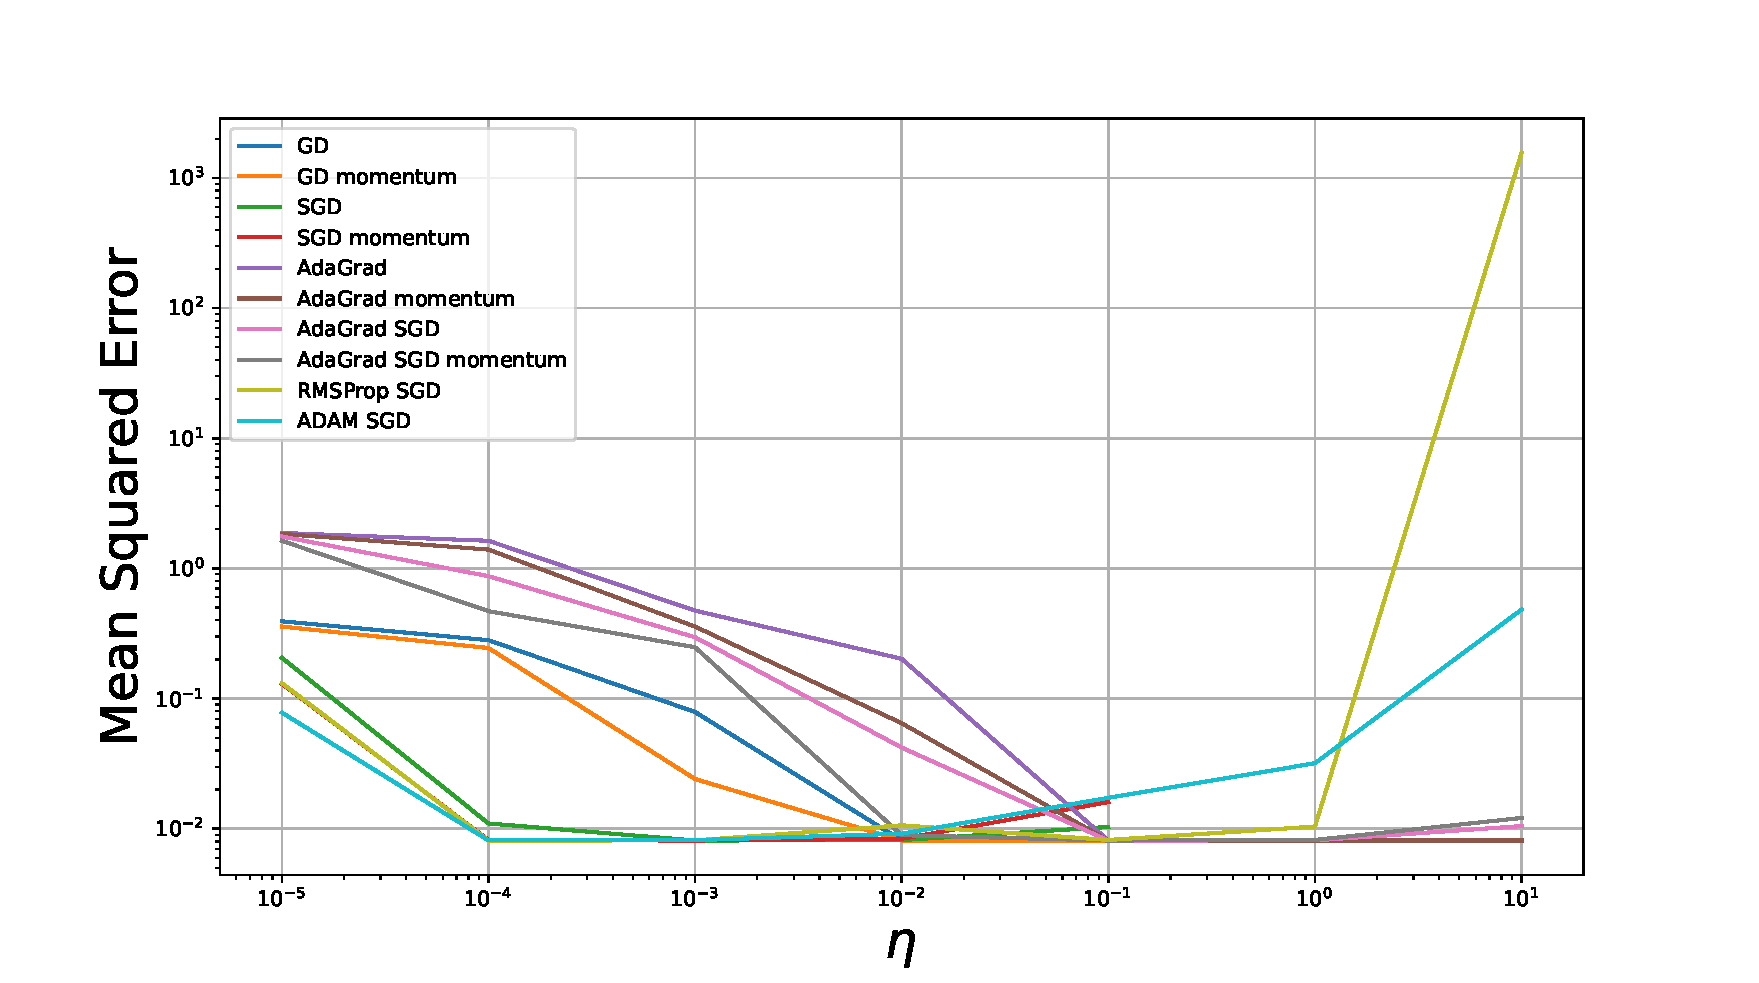
\includegraphics[width=0.91\linewidth]{images/error_vs_learningrate.pdf}
    \caption{MSE as a function of learning rate $\eta$, for all implemented gradient methods.}
    \label{fig:error_vs_learningrate}
\end{figure}

We start off by presenting an overview for all gradient descent methods implemented in \autoref{fig:error_vs_learningrate}. The evaluation metric shown is the mean squared error, expressed in \autoref{eq:mse}. This is plotted against learning rate on the x-axis, which can then be used to choose suitable learning rates for the various gradient descent methods.

\begin{figure}
    \centering
    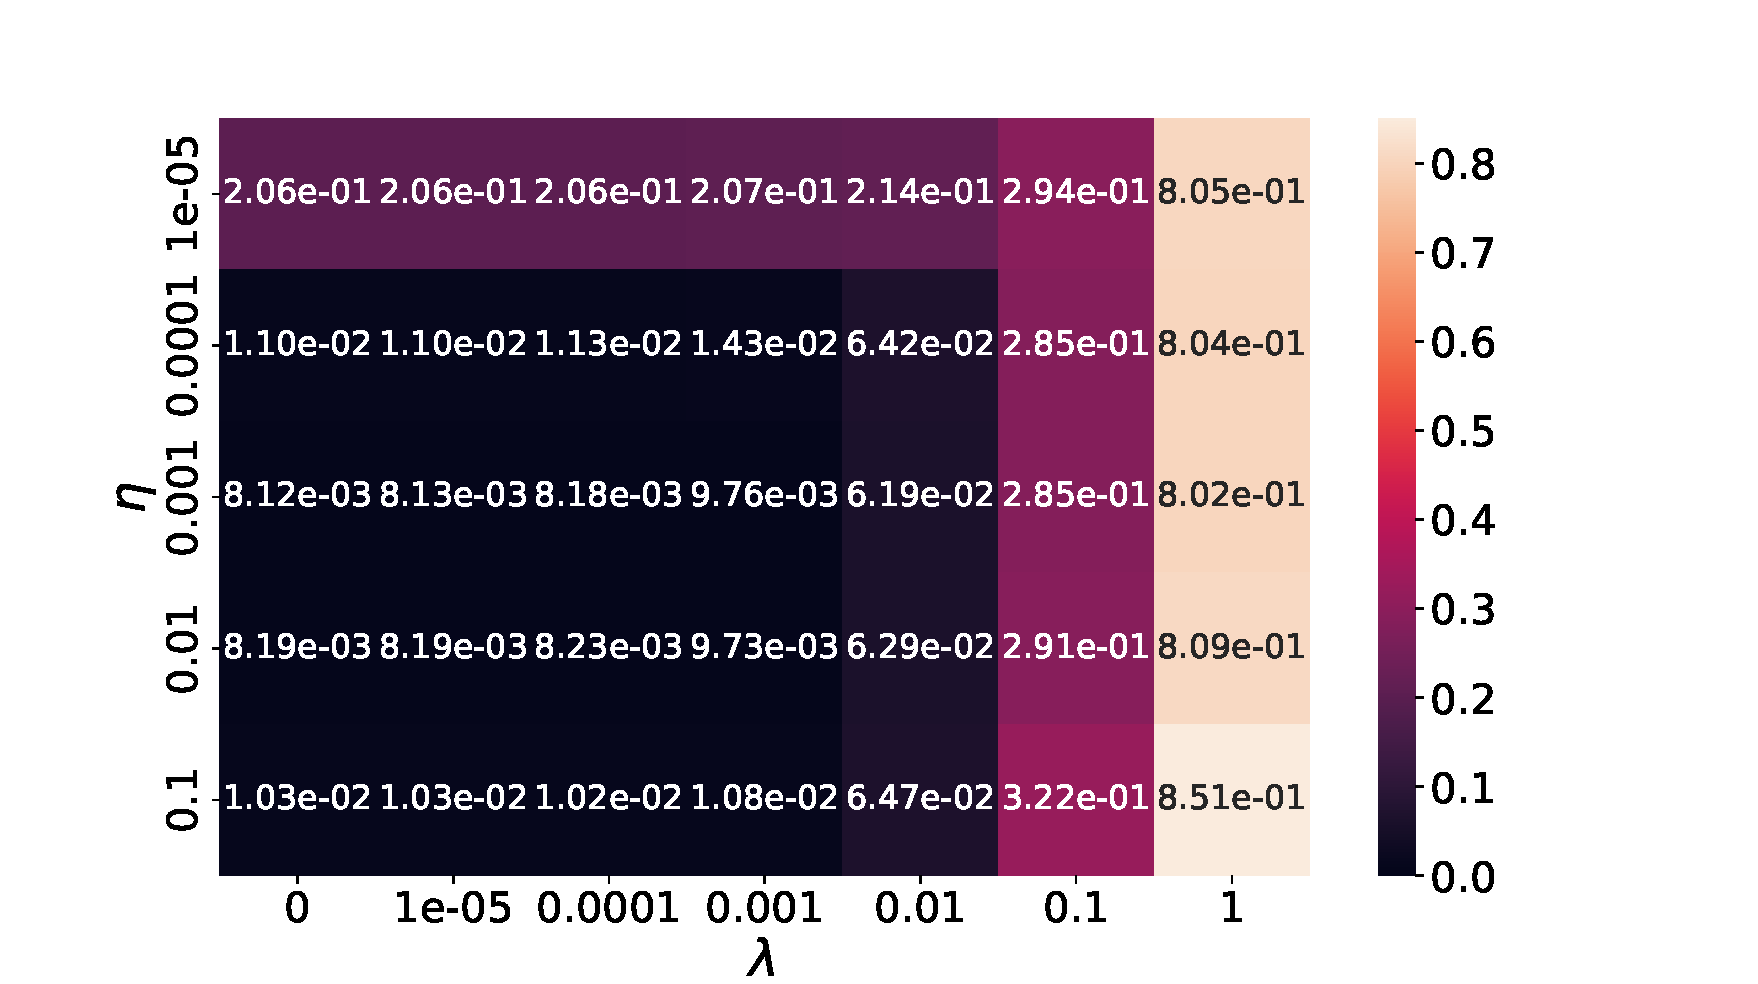
\includegraphics[width=0.91\linewidth]{images/eta_vs_lambda_SGD.pdf}
    \caption{Mean squared error as a function of learning rate $\eta$ and regularization parameter $\lambda$, for stochastic gradient descent with batch size = 5.}
    \label{fig:eta_vs_lambda_SGD}
\end{figure}

Next, to investigate the relationship between different parameters more closely, we focus on the stochastic gradient descent (SGD) algorithm, while varying the relevant parameters. In \autoref{fig:eta_vs_lambda_SGD}, the mean squared error is shown as a function of both the learning rate $\eta$, and the regularization parameter $\lambda$. This figure shows a general trend of no regularization performing the best, coupled with a medium learning rate, i.e. the results get worse when the learning rate approaches either 1 or 0. 

\begin{figure}
    \centering
    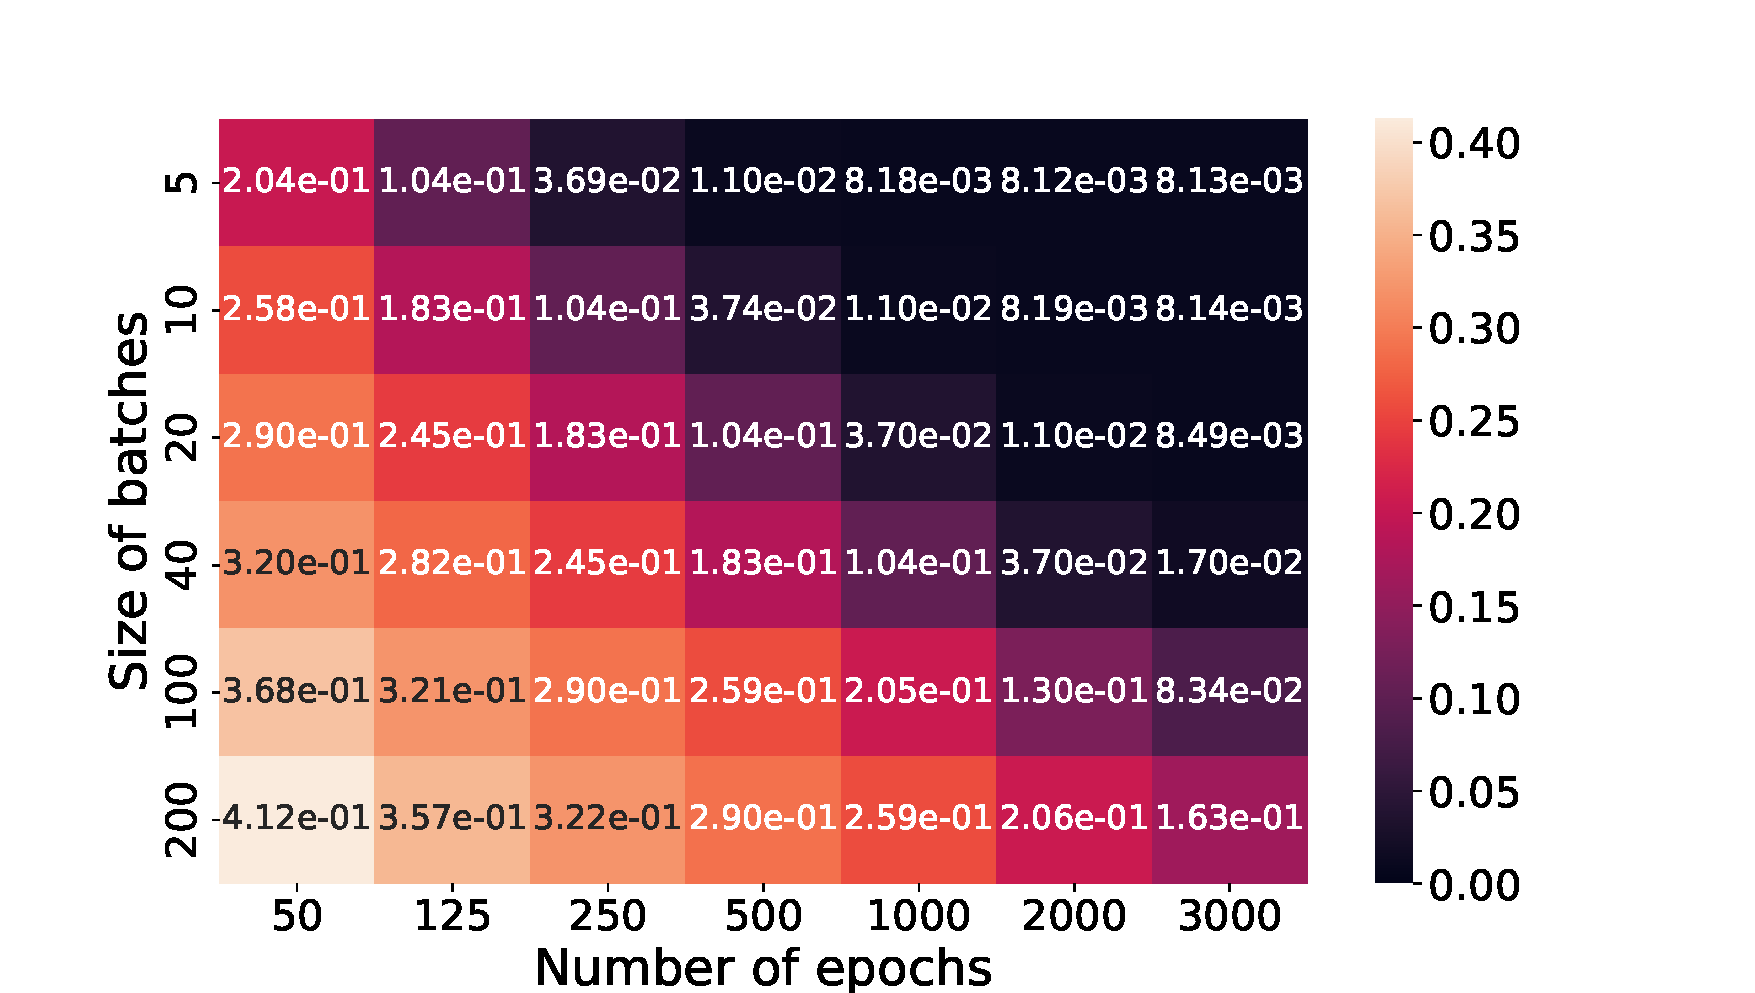
\includegraphics[width=0.91\linewidth]{images/batch_vs_epochs_SGD.pdf}
    \caption{Mean squared error as a function of batch size and number of epochs, for the stochastic gradient descent algorithm, with learning rate $\eta = 10^{-3}$ and regularization parameter $\lambda = 0$.}
    \label{fig:batch_vs_epochs_SGD}
\end{figure}

\autoref{fig:batch_vs_epochs_SGD} displays the mean squared error as a function of the batch size and the number of epochs in the SGD algorithm. Unsurprisingly, the error decreases as a function of epochs as long as the model does not overfit the training data. Meanwhile, the results show that you can achieve faster convergence for a smaller number of epochs by decreasing the batch size.%, as this causes an increase in the number of updates in the model parameters during an epoch. 

\begin{figure}
    \centering
    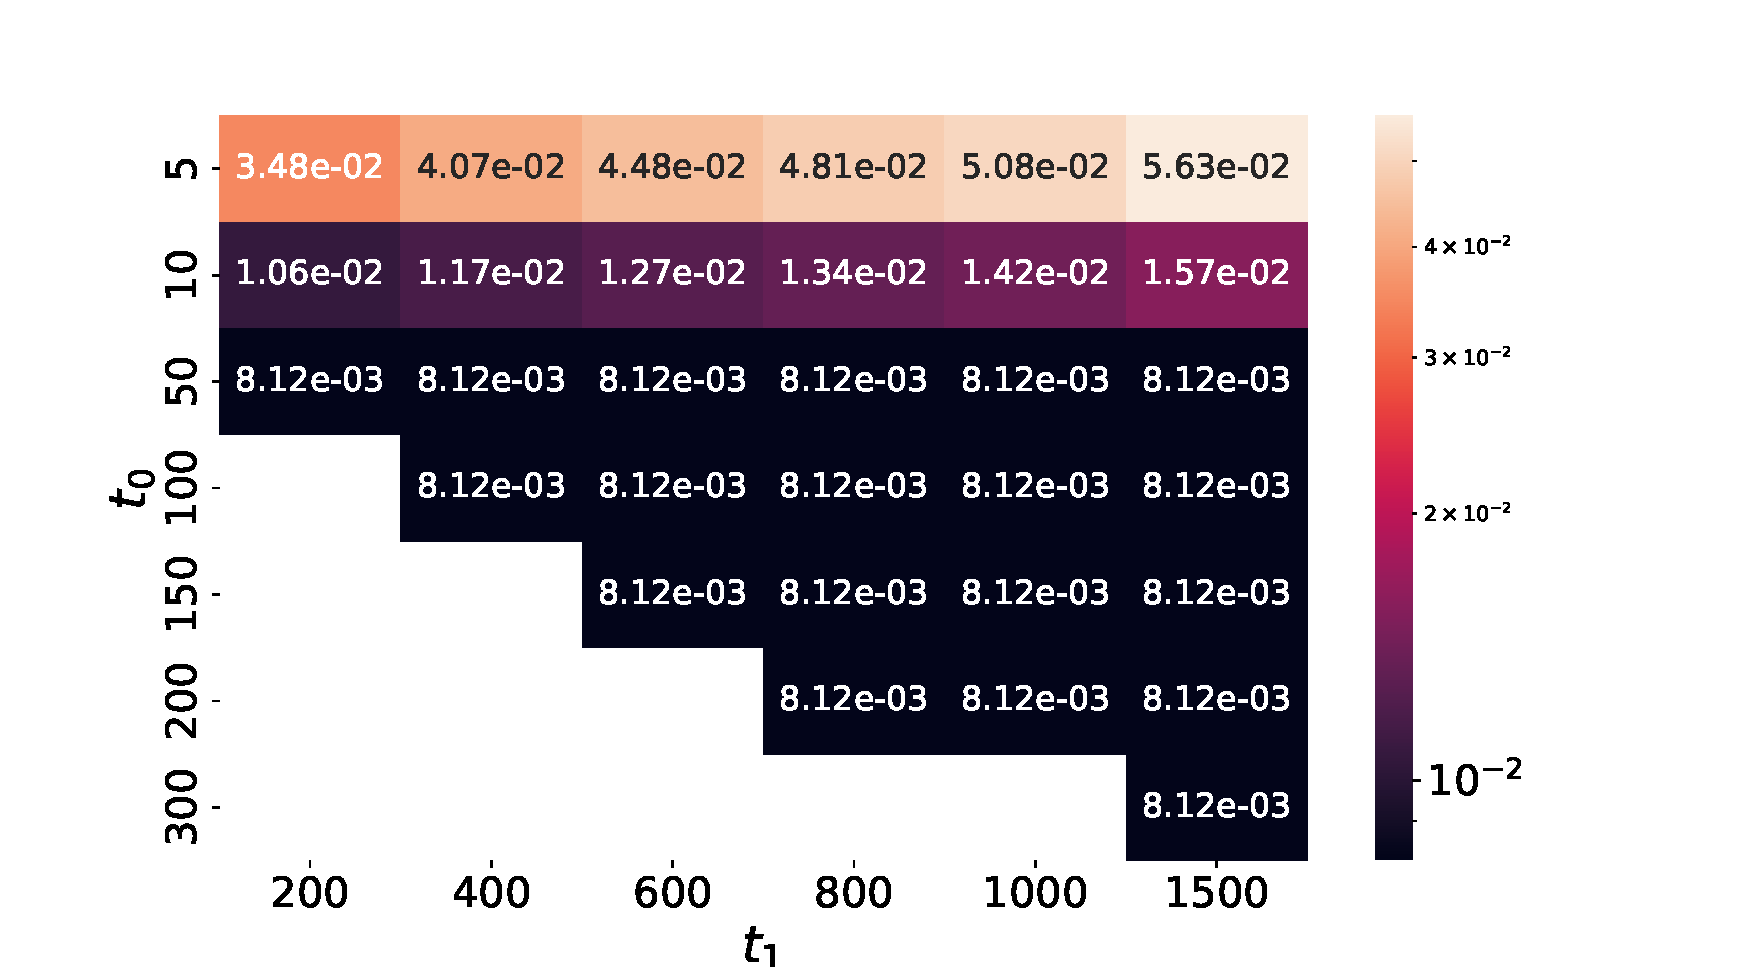
\includegraphics[width=0.91\linewidth]{images/t0_t1.pdf}
    \caption{Mean squared error shown as a function of the hyperparameters $t_0$ and $t_1$, used for tuning the learning rate with time decay in the SGD algorithm. The SGD was run with regularization parameter $\lambda = 0$. The values which diverge are masked.}
    \label{fig:t0_t1}
\end{figure}

Next, we present the results of tuning the time decay parameters $t_0$ and $t_1$ in \autoref{fig:t0_t1}, for scaling the learning rate. We found the best results to be given by $t_0 > 50$, and $t_1 > 200$. Combinations of values where the fraction $\frac{t_1}{t_0}$ approached 3 or below lead to exploding gradients, and were discarded as a viable options. 

\begin{figure}
    \centering
    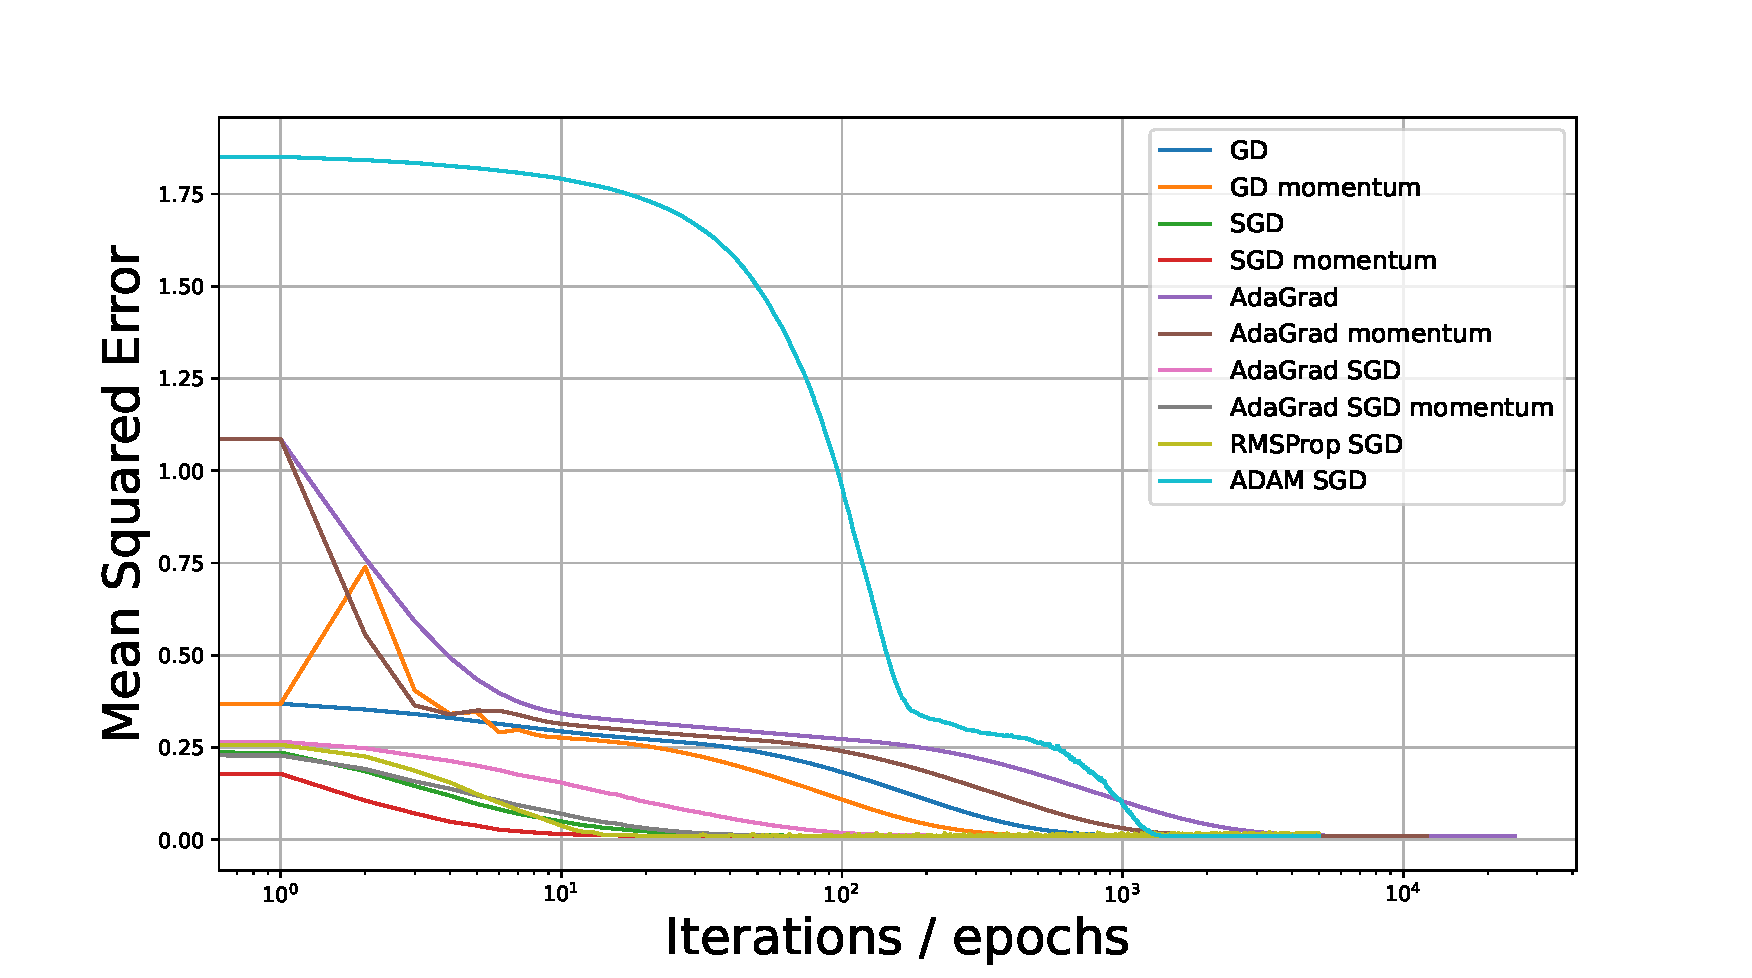
\includegraphics[width=0.91\linewidth]{images/error_vs_iteration_semilogx.pdf}
    \caption{Mean squared error as a function of number of iterations/epochs. The parameters used, which we found to be reasonable from the results in Figs. \ref{fig:error_vs_learningrate}, \ref{fig:eta_vs_lambda_SGD}, \ref{fig:batch_vs_epochs_SGD}, \ref{fig:t0_t1} and experience while testing, are summarized in Table \ref{tab:GD_params}.}
    \label{fig:error_vs_iteration_semilogx}
\end{figure}

In \autoref{fig:error_vs_iteration_semilogx} we present the mean squared error as a function of number of iterations/epochs. This provides insight into how fast the gradient descent methods converge. One important point to consider is that this does not show actual computational time, or floating point operations (FLOPS), since each method does different operations within one iteration. Still, \autoref{fig:error_vs_iteration_semilogx} provides decent grounds for comparison between methods at a surface level, gives an estimate of how many iterations each method needs individually, and a measure of how well each method has converged. The parameters used to produce \autoref{fig:error_vs_iteration_semilogx} are tabulated in Table \ref{tab:GD_params}, and were found to be reasonable parameters for these methods overall. 

\begin{table}
    \centering
    \caption{Parameters for the gradient methods shown in \autoref{fig:error_vs_iteration_semilogx}.}
    \begin{center}
    \begin{tabular}{ |c|c c c c c c c c| } 
    \hline
    Method & $\eta$ & $\lambda$ & $\gamma$ & M & $t_0$ & $t_1$ & $\rho_1$ & $\rho_2$ \\
    \hline
    GD & 0.1 & 0 & - & - & - & - & - & -\\ 
    GD /w mom & 0.1 & 0 & 0.5 & - & - & - & -& -\\
    SGD & - & 0 & - & 5 & 50 & 1500 & -& - \\
    SGD /w mom & - & 0 & 0.5 & 5 & 50 & 1500 & -& -\\ 
    AdaGrad & 0.1 & 0 & - & - & - & - & -& -\\
    AdaGrad /w mom & 0.1 & 0 & 0.5 & - & - & - & -& -\\
    AdaGrad SGD & 0.1 & 0 & - & 5 & - & -& -& -\\ 
    AdaGrad SGD /w mom & 0.1 & 0 & 0.5 & 5 & - & - & -& -\\
    RMSProp SGD & 0.01 & 0 & - & 5 & - & - & 0.99 & -\\
    ADAM SGD & 0.001 & 0 & - & 5 & - & - & 0.9 & 0.999\\
    \hline
    \end{tabular}
    \end{center}
    \label{tab:GD_params}
\end{table}


\begin{figure}
    \centering
    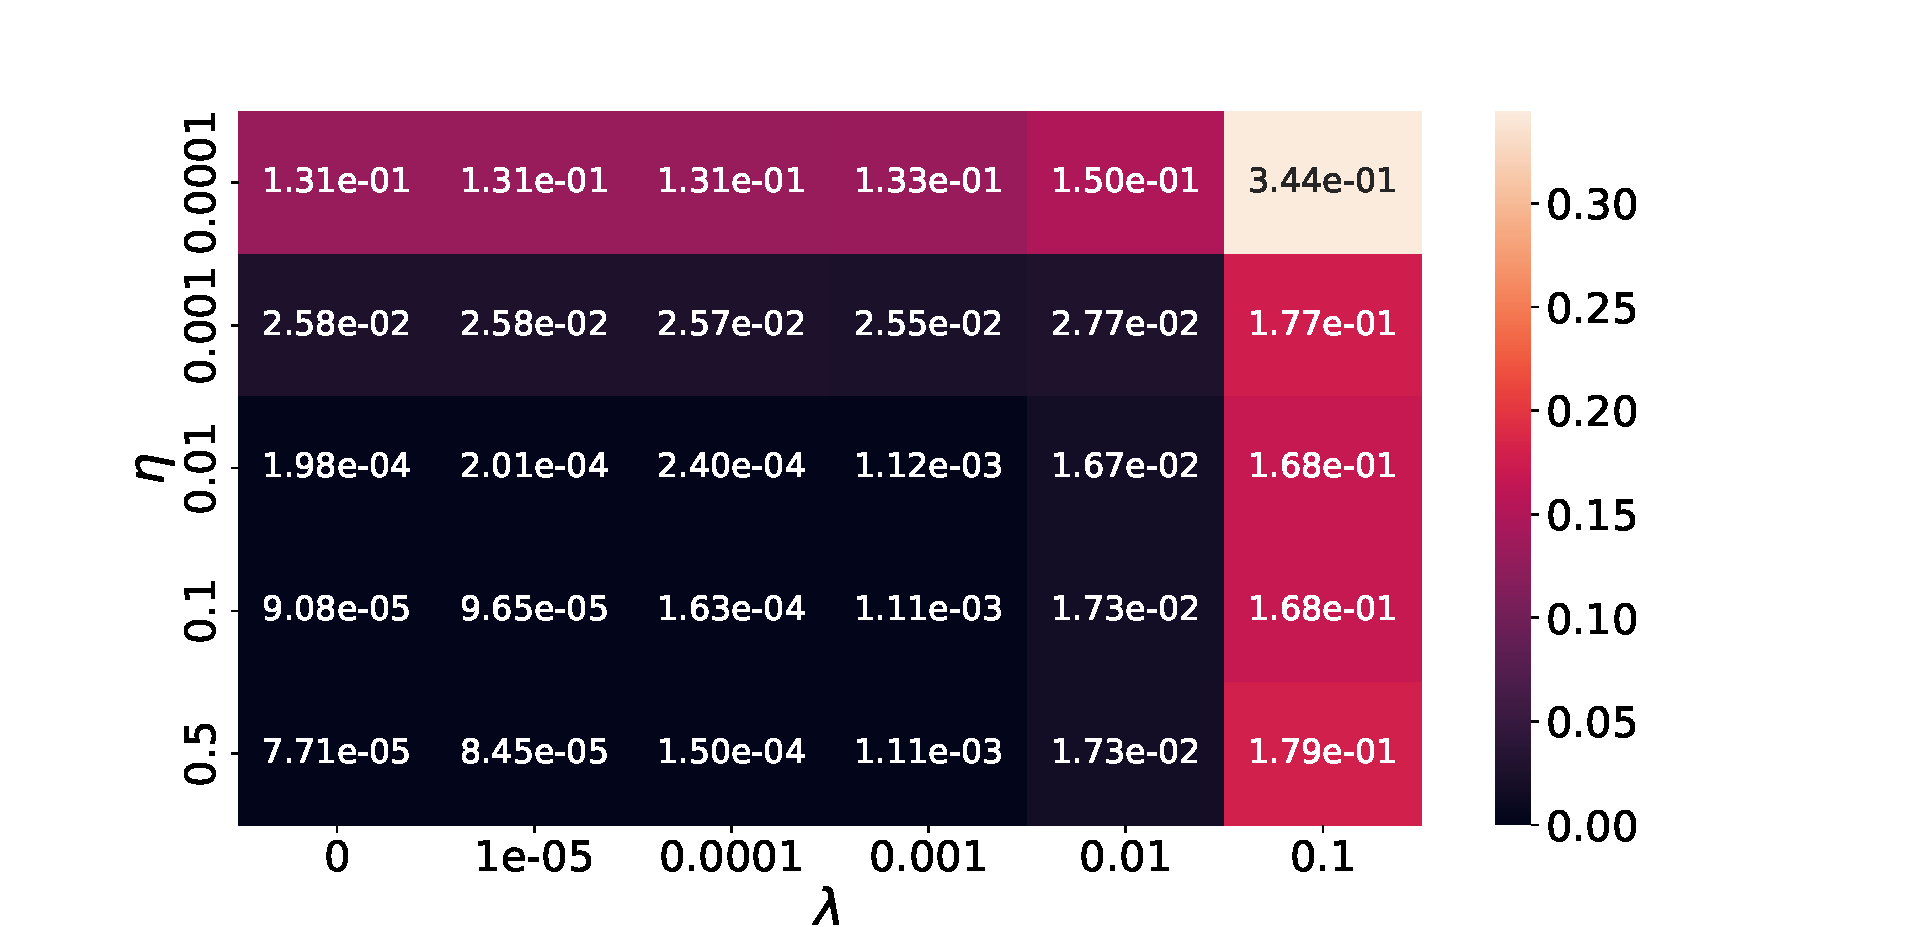
\includegraphics[width=0.91\linewidth]{images/mse_NN_eta_vs_lambda.pdf}
    \caption{Mean squared error for regression, as a function of learning rate $\eta$ and regularization parameter $\lambda$. This neural network had one hidden layer with three nodes, sigmoid activation function for the hidden layer, and linear activation for the output layer.}
    \label{fig:mse_NN_eta_vs_lambda}
\end{figure}

Next, we present the results from our neural network. First, mean squared error (MSE) for linear regression are shown in \autoref{fig:mse_NN_eta_vs_lambda}. These results were produced with a neural network of one hidden layer with sigmoid activation, containing three nodes. For the output layer, we chose linear activation, that is $f(x) = x$. The MSE is shown as a function of both learning rate $\eta$, and L2-regularization parameter $\lambda$. Linear regression with gradient descent methods, and in project 1, without regularization ($\lambda = 0$) corresponding to ordinary least squares (OLS), performed the best. For the neural network, the best results were produced with a "medium" learning rate, that is not approaching either 0 or 1. A learning rate of $\eta \geq 1$ again produced exploding gradients. 

\begin{figure}
    \centering
    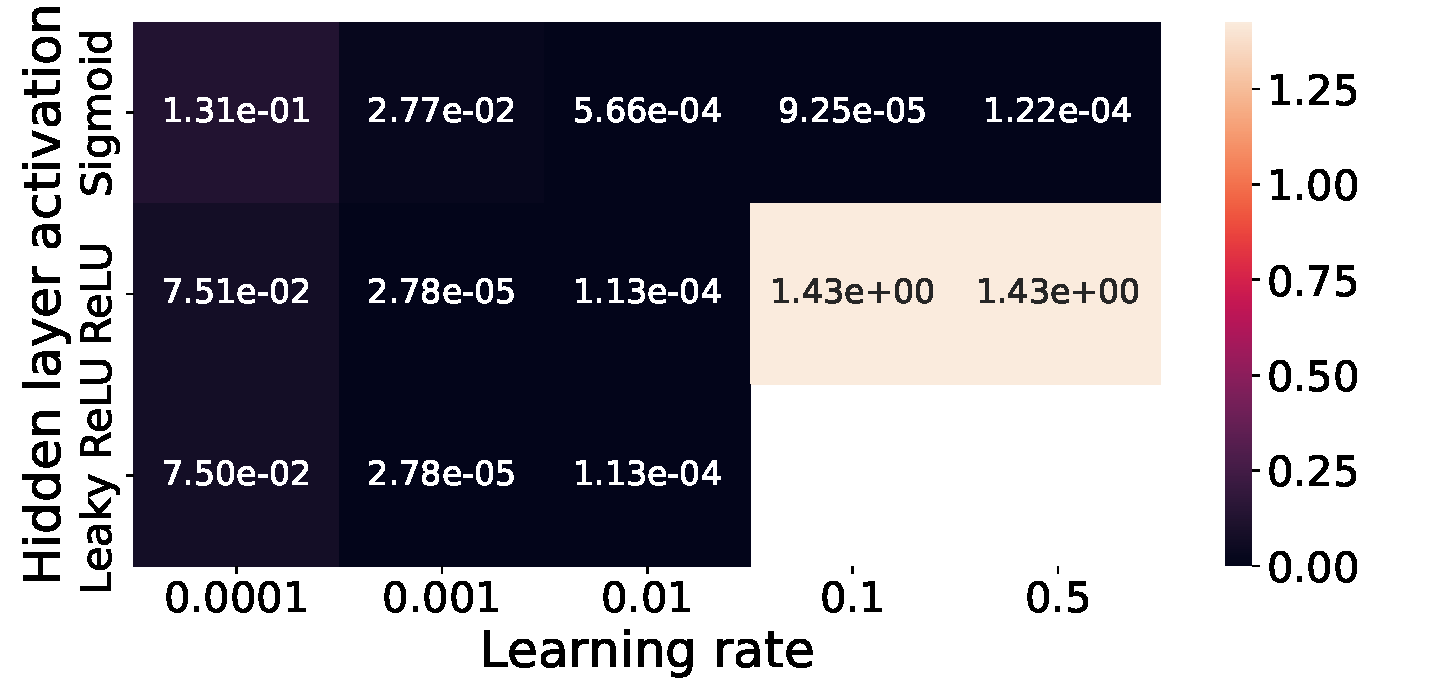
\includegraphics[width=0.91\linewidth]{images/mse_NN_activation_vs_eta.pdf}
    \caption{Mean squared error for regression, as a function of learning rate $\eta$ and activation function in the hidden layers. This neural network had one hidden layer with three nodes, and linear activation for the output layer. The leaky ReLU had a leakage coefficient of $\alpha = 0.01$. The diverging MSE values are shown as blank.}
    \label{fig:mse_NN_activation_vs_eta}
\end{figure}

In \autoref{fig:mse_NN_activation_vs_eta}, we show the MSE as a function of activation function in the hidden layer, as well as learning rate $\eta$. This is run with regularization parameter $\lambda = 0$. For the case of leaky ReLU, the leakage coefficient was $\alpha = 0.01$, as defined in \autoref{eq:leaky_relu}. The best results were found for ReLU and leaky ReLU with learning rate $\eta = 0.001$, being equally accurate. We achieved slightly worse, but comparable, precision using sigmoid activation, but for higher learning rate $\eta = 0.1$. Learning rates at 0.1 or above gave poor results for both ReLU and leaky ReLU.

\begin{figure}
    \centering
    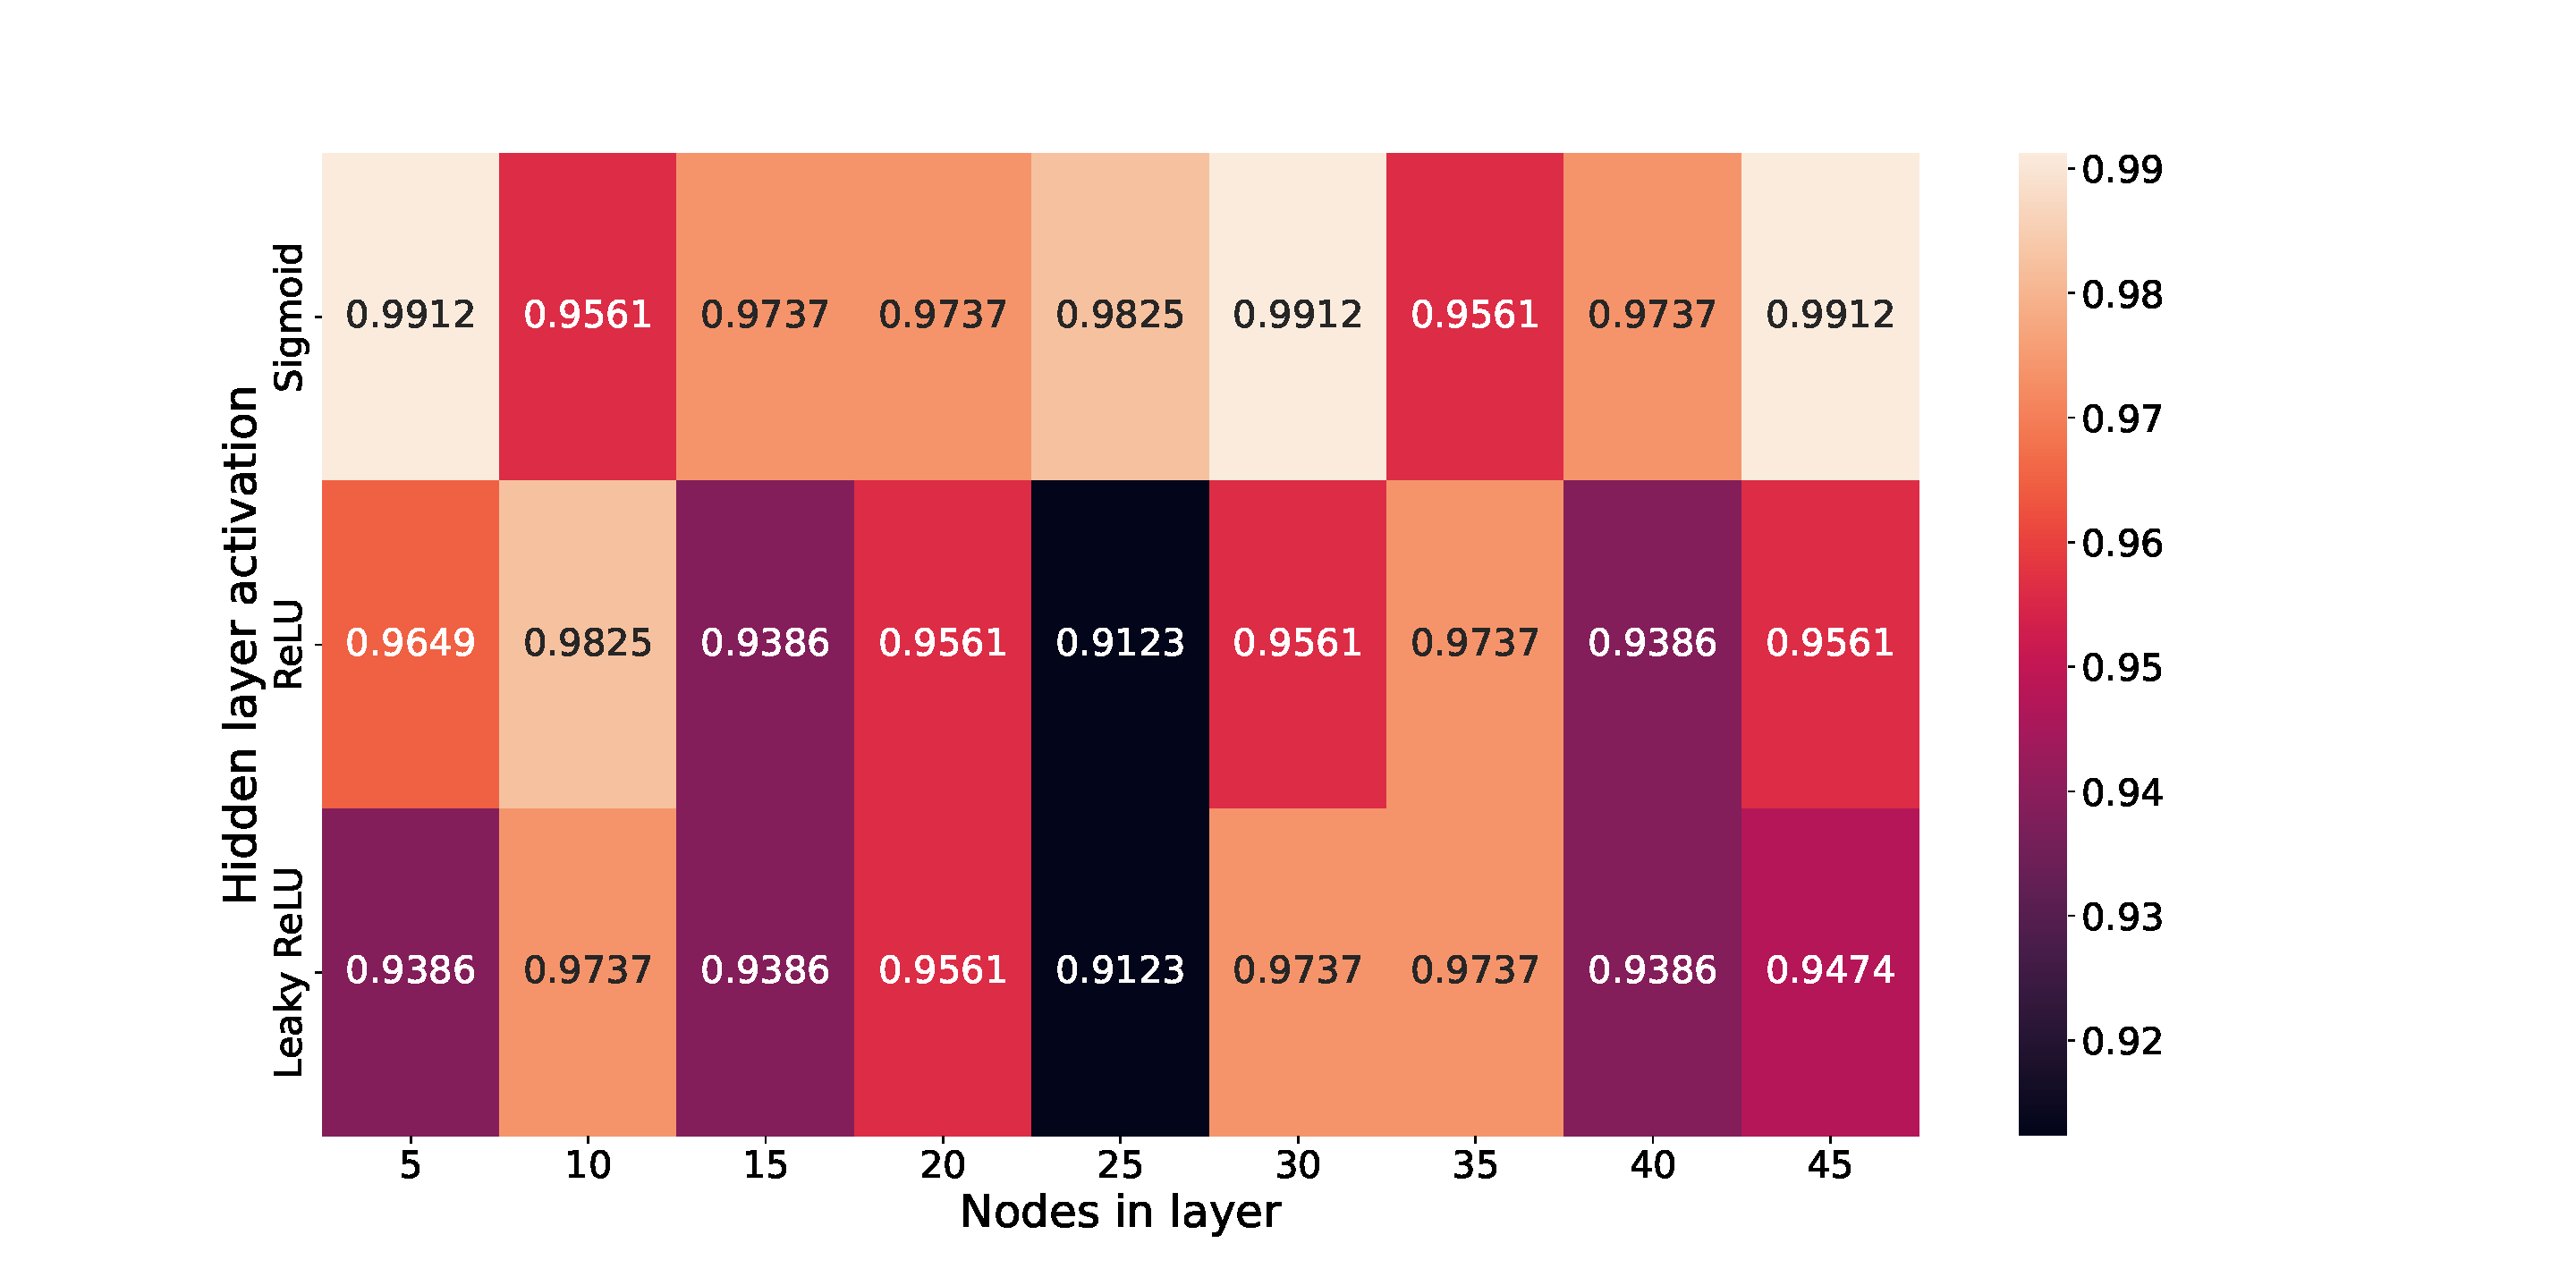
\includegraphics[width=\textwidth]{images/accuracy_activations_and_nodes_fixed_eta.pdf}
    \caption{Accuracy score for classification of the Wisconsin breast cancer data set using a neural network with a single hidden layer, for different configurations of activation function and number of nodes in the hidden layer. The leaky ReLU activation given by the expression in \autoref{eq:leaky_relu} was used with a leakage parameter $\alpha=0.01$.}
    \label{fig:nn_class_one_layer_activations}
\end{figure}

We now present the results for classification, for both the neural net and logistic regression. We start off by presenting the accuracy score, given by \autoref{eq:acc_score}, for a single hidden layer neural network in \autoref{fig:nn_class_one_layer_activations}. The accuracy is shown as a function of number of nodes and type of activation function in the hidden layer. For classification, the sigmoid activation function performs very well, reaching an accuracy of \SI{99.12}{\%} for multiple configurations of nodes. However, it can be seen that all configurations perform well, with the lowest achieved accuracy score being \SI{91.23}{\%} for ReLU and leaky ReLU with 25 nodes. 

\begin{figure}
    \centering
    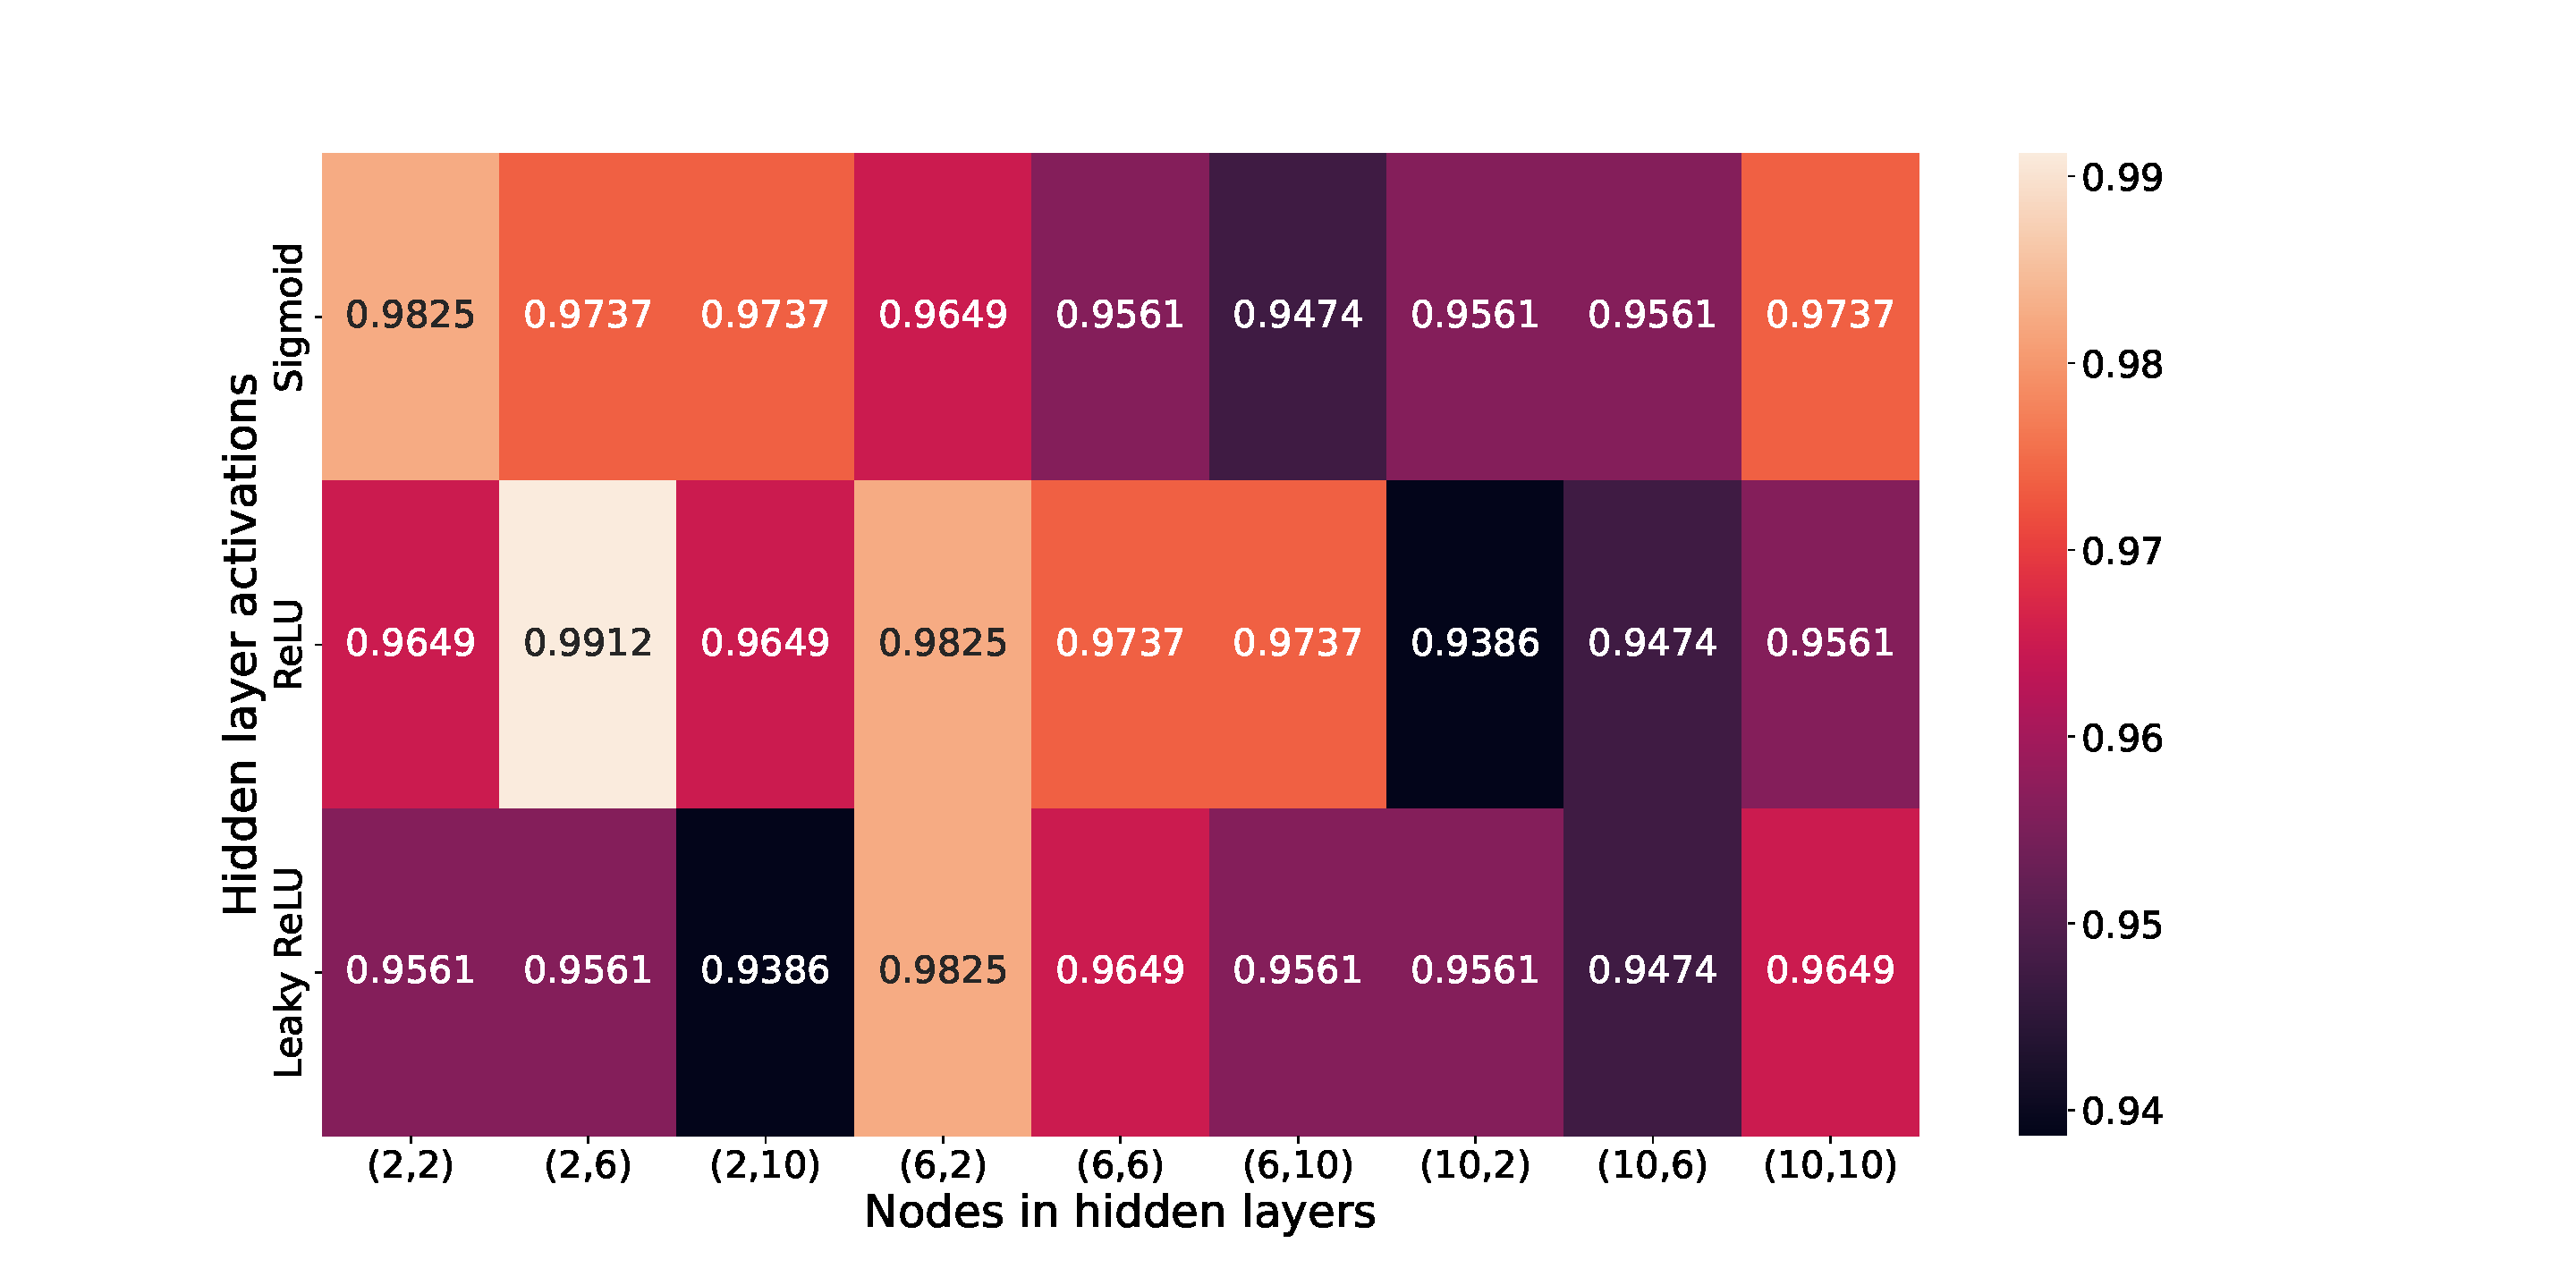
\includegraphics[width=0.91\linewidth]{images/accuracy_activations_and_two_layers_fixed_eta.pdf}
    \caption{Accuracy score for classification of breast cancer data, in a two hidden layer neural net, for different configurations of activation function and number of nodes in the hidden layers. The tuples on the x-axis denote the number of nodes in (layer1, layer2). The leaky ReLU activation given by the expression in \autoref{eq:leaky_relu} was used with a leakage parameter $\alpha=0.01$.}
    \label{fig:nn_class_two_layer_activations}
\end{figure}

A similar plot is shown in \autoref{fig:nn_class_two_layer_activations}, but now with two hidden layers. The tuples on the x-axis denote the number of nodes in the hidden layer, i.e. (6,10) represents 6 nodes in the first hidden layer and 10 nodes in the second hidden layer. In contrast to the results in \autoref{fig:nn_class_one_layer_activations}, the ReLU activation function achieves the highest accuracy score, with $99.12\%$ accuracy. Again, every combination performs well, with the lowest accuracy score being \SI{93.86}{\%} for combinations (ReLU, (10,2)) and (leaky ReLU, (2,10)). 

\begin{figure}
    \centering
    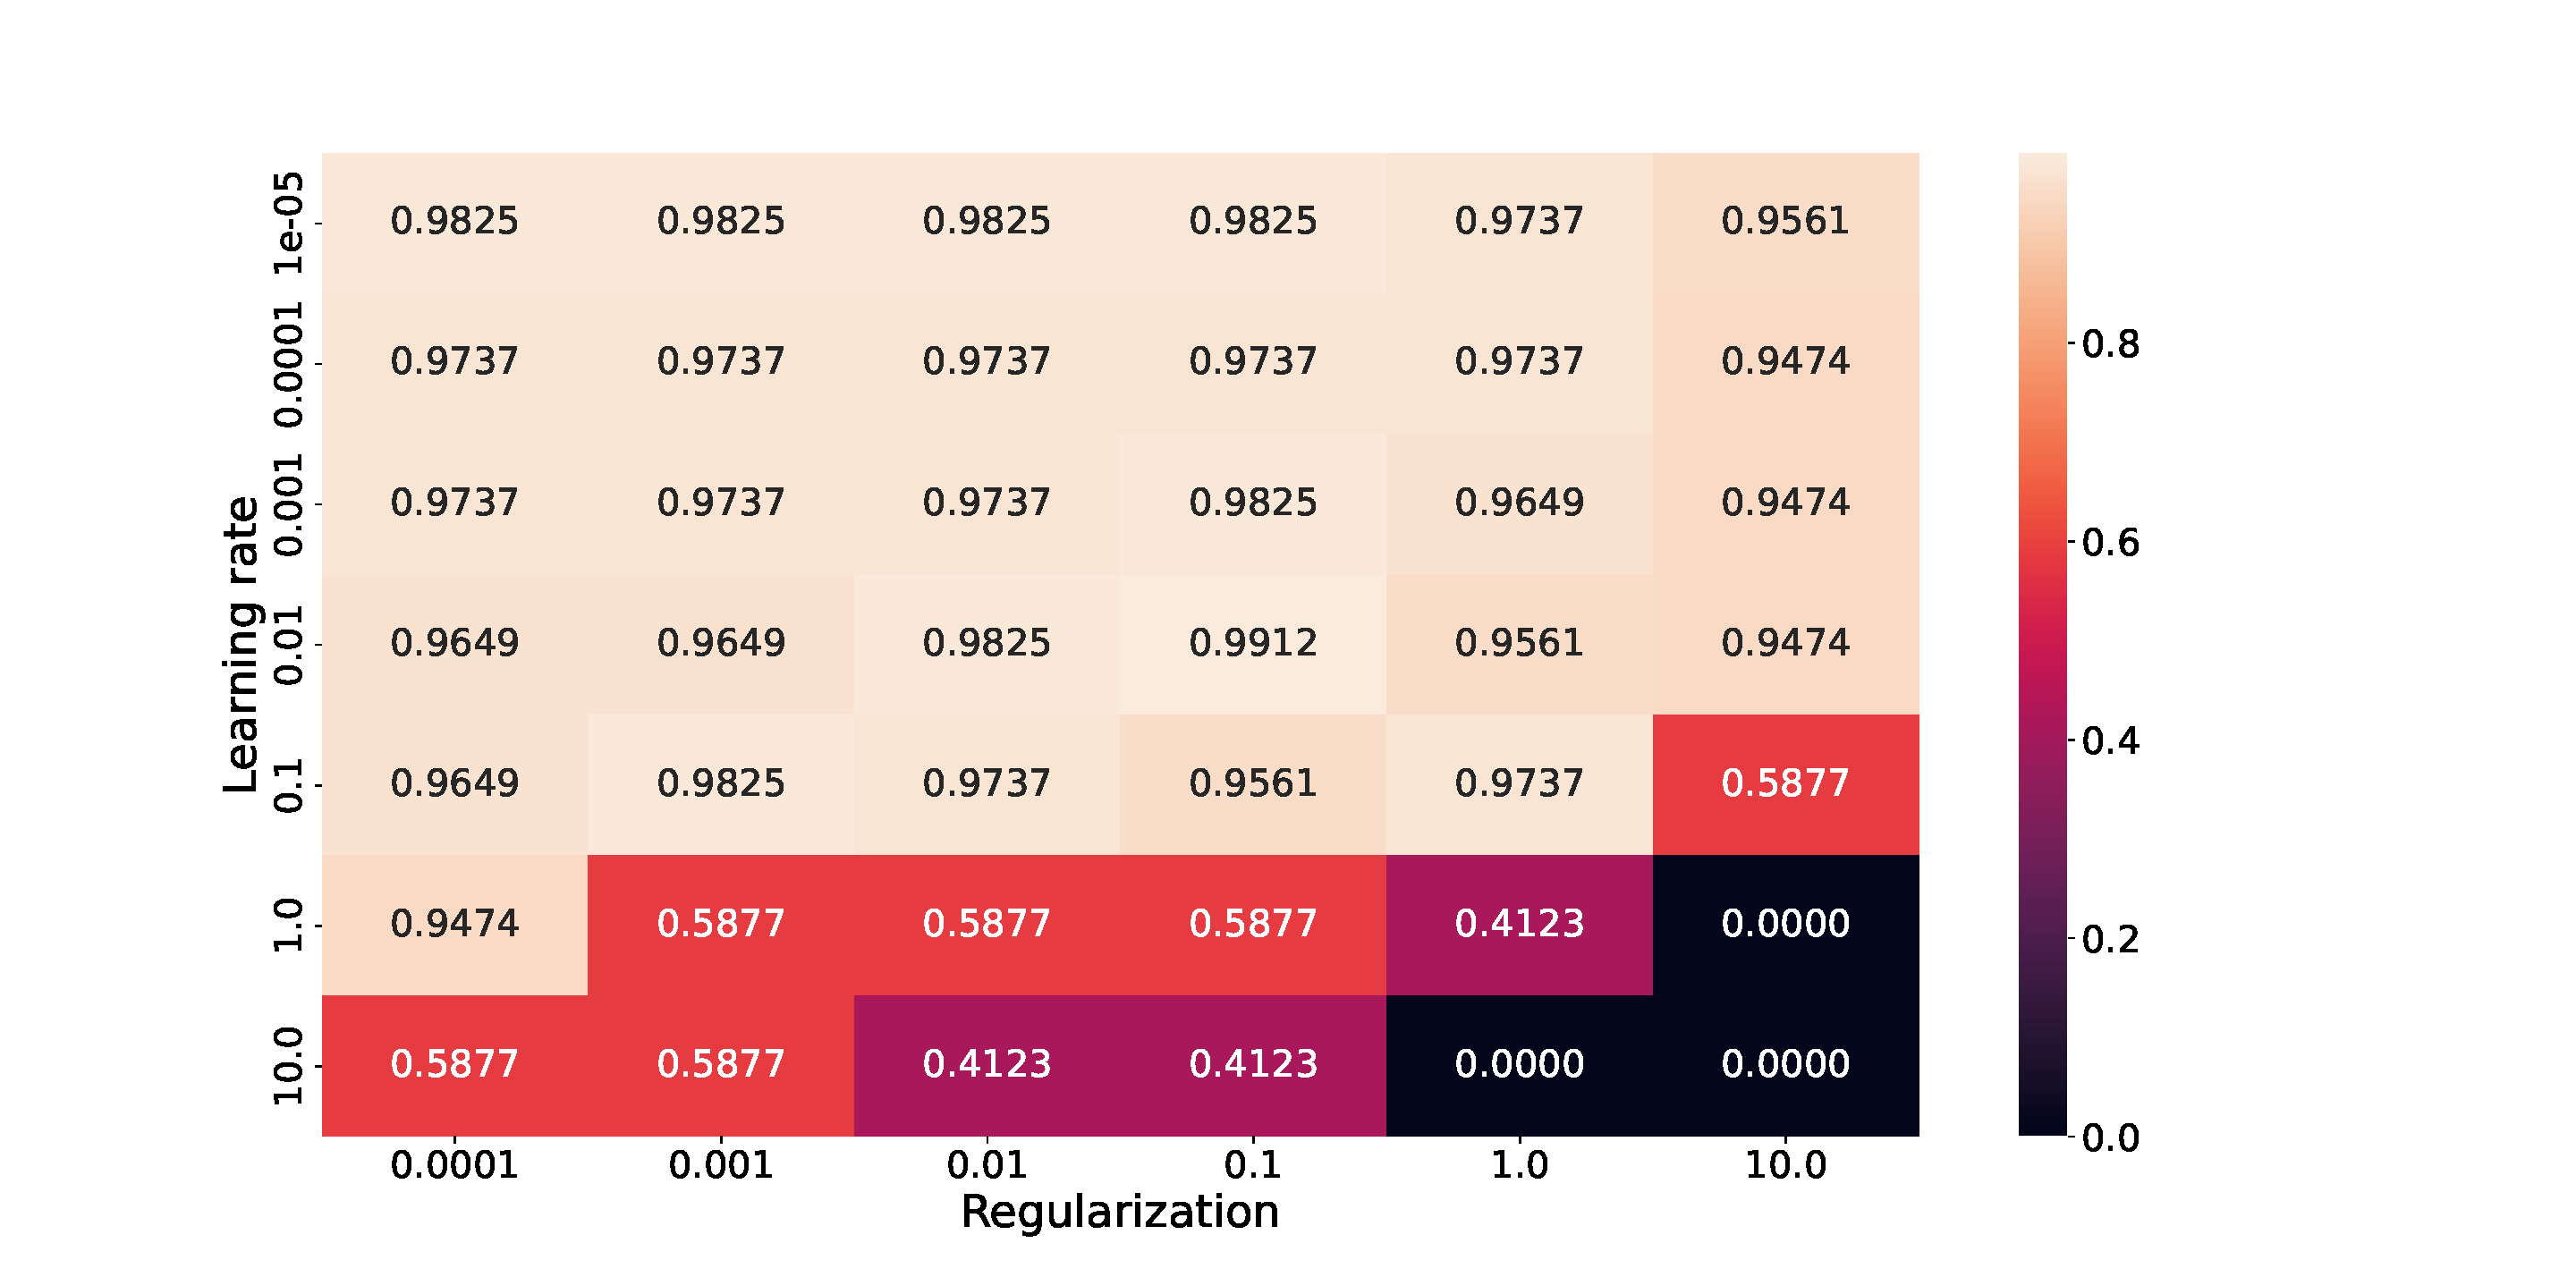
\includegraphics[width=0.91\linewidth]{images/regularization_vs_learning_rate_20_nodes_fixed_learning_1000_epochs.pdf}
    \caption{Accuracy score for classification of the Wisconsin breast cancer data set using in a single hidden layered neural network with 20 nodes in the hidden layer, as a function of learning rate $\eta$ and regularization parameter $\lambda$. The models were trained using stochastic gradient descent for 1000 epochs with 10 minibatches created by splitting the training data. Combinations with \SI{0}{\%} accuracy is models where the calculations diverged.}
    \label{fig:nn_class_lambda_vs_eta}
\end{figure}


\begin{figure}
    \centering
    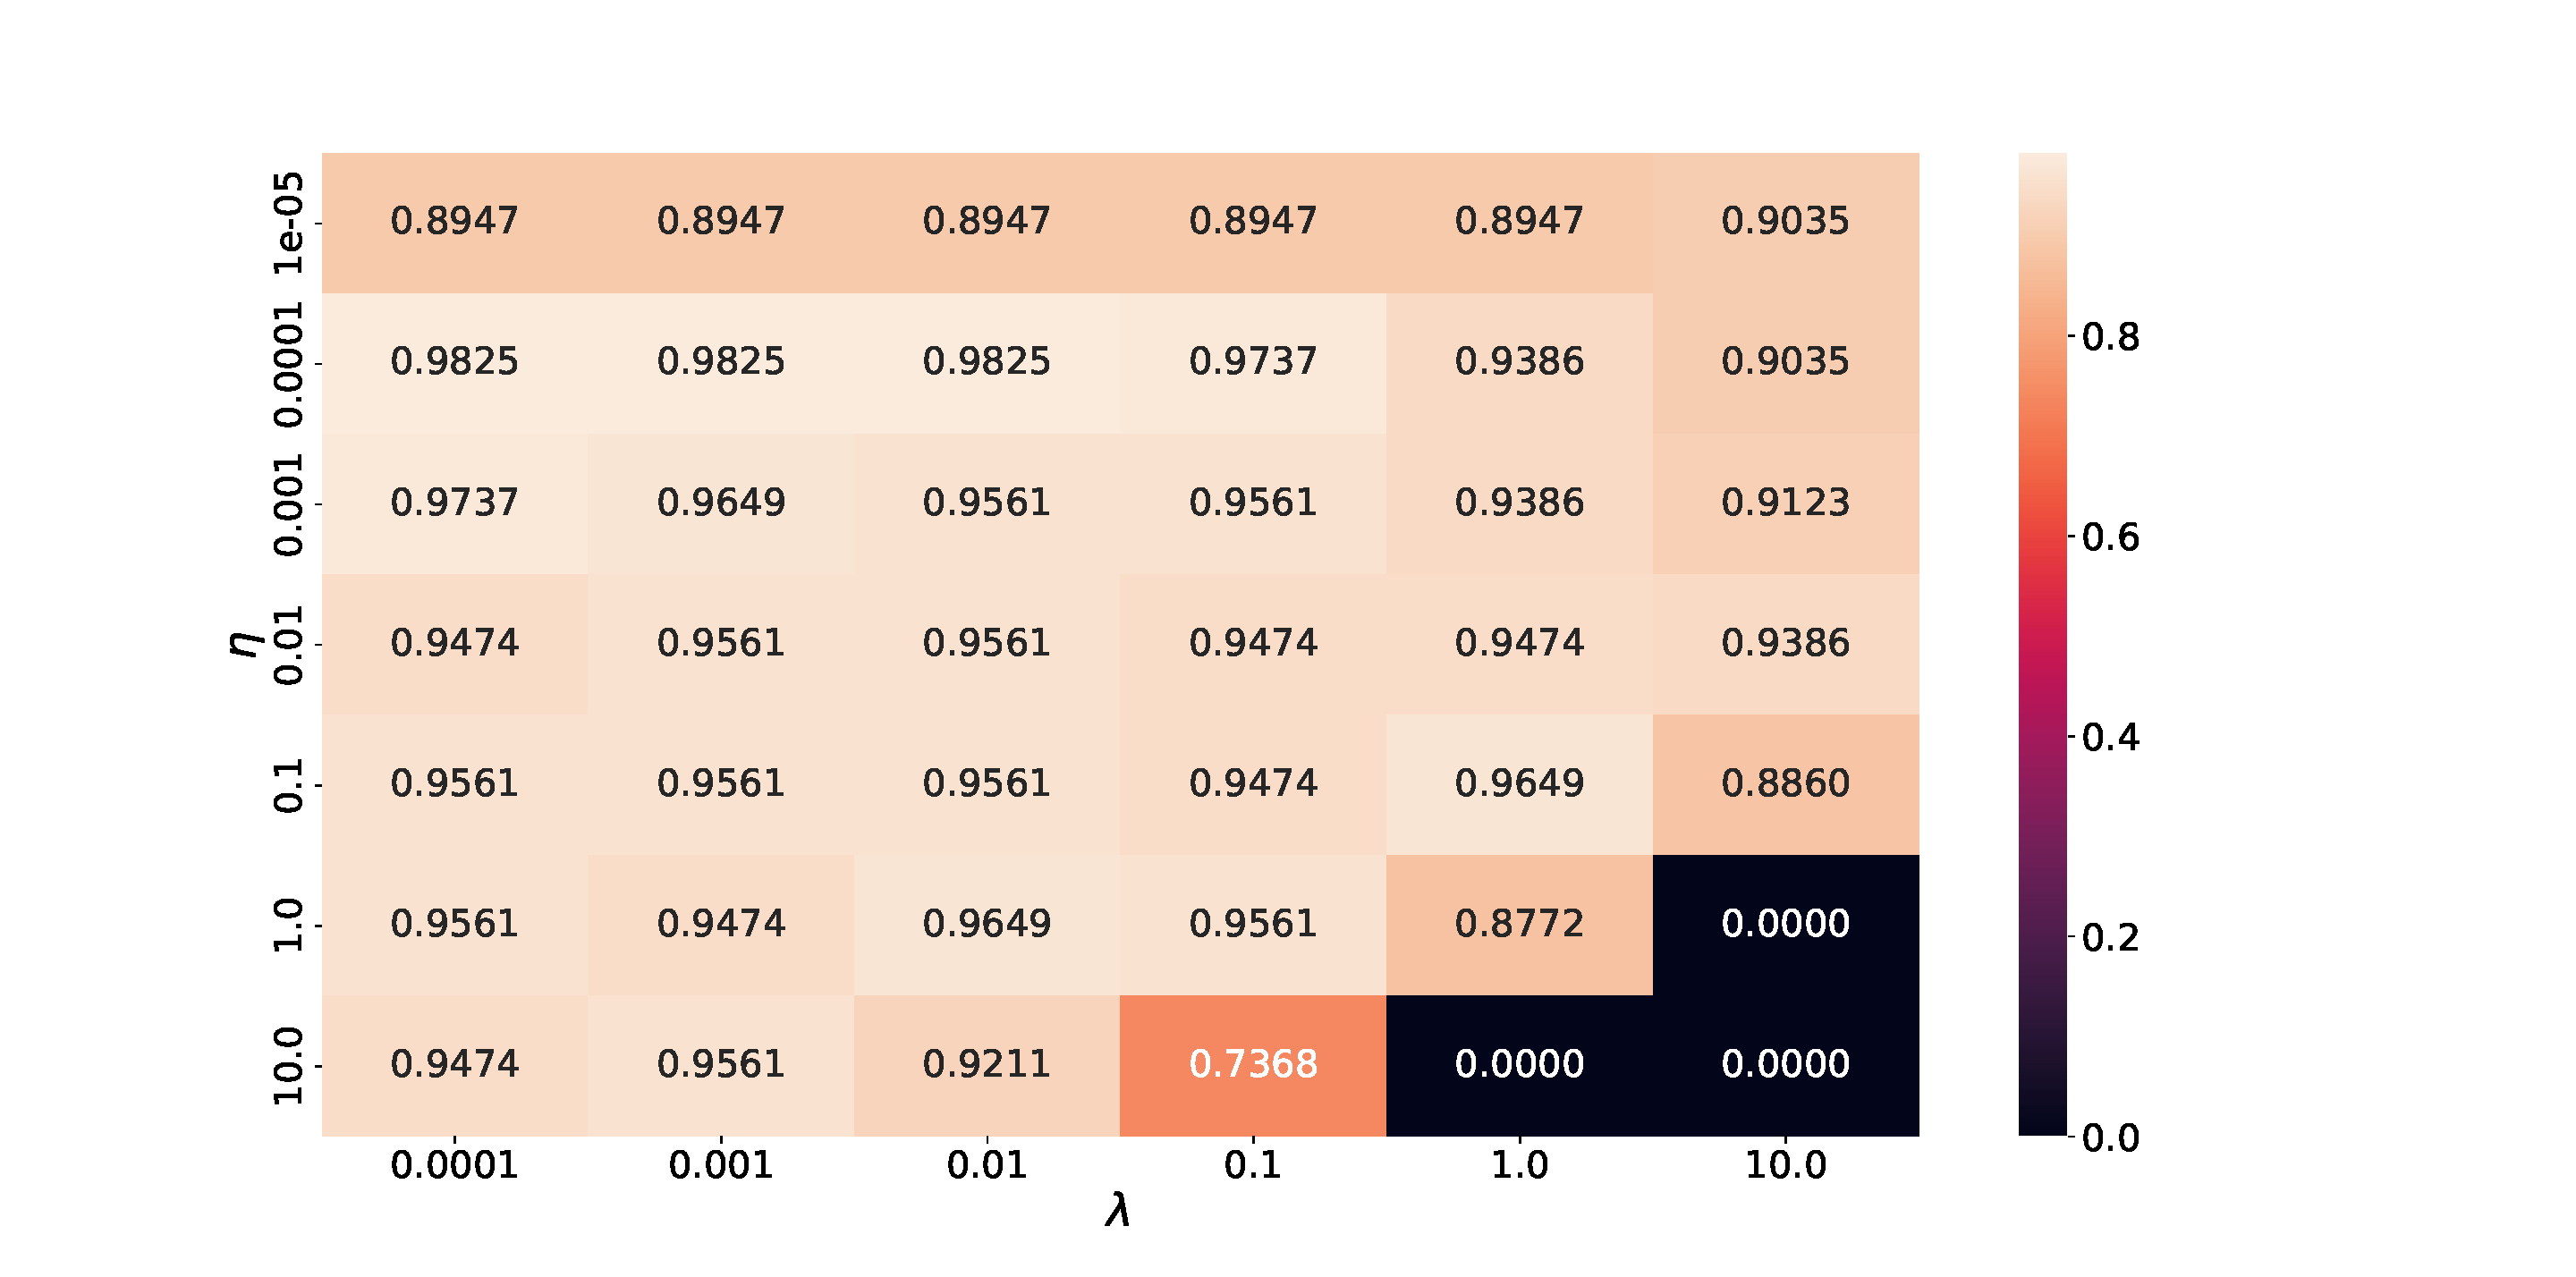
\includegraphics[width=0.91\linewidth]{images/logreg_regularization_vs_learning_rate_fixed_learning_1000_epochs.pdf}
    \caption{Accuracy score for classification of the Wisconsin breast cancer data set using logistic regression as a function of learning rate $\eta$ and regularization parameter $\lambda$. The models were trained using stochastic gradient descent on 10 minibatches for 1000 epochs. Combinations with \SI{0}{\%} accuracy is models where the calculations diverged.}
    \label{fig:log_class_lambda_vs_eta}
\end{figure}

Finally, two plots comparing accuracy score for a neural network and logistic regression are shown in \autoref{fig:nn_class_lambda_vs_eta} and \autoref{fig:log_class_lambda_vs_eta} respectively. The accuracy score is shown as a function of learning rate $\eta$ and regularization parameter $\lambda$. The darkest squares of \SI{0}{\%} correct predictions show combinations of learning rate and regularization which did not converge. Generally, the neural network seems to achieve slightly better accuracy than logistic regression, but performs worse at higher learning rates. Logistic regression seems more robust to most combinations of hyperparameters. 

\section{Discussion} \label{sec:discussion}
When we compared the different gradient descent methods, SGD and SGD with momentum coupled with an adaptive time decay learning rate seemed to provide solid results while being relatively simple to tune. SGD and SGD with momentum also provided a significant speedup as compared to their regular gradient descent counterparts. More complicated methods like AdaGrad and ADAM did not provide a significant improvement on the results. This, perhaps, because of the low complexity of the problem. RMSProp yielded fast convergence, but both RMSProp and ADAM displayed small oscillations around the desired solution at the end, while the other methods provided a more stable convergence, as seen in \autoref{fig:error_vs_iteration_semilogx}.

Generally, we found that the learning rates giving the best results were in the range $\eta \in \left[10^{-3}, 10^{-1}\right]$, for both linear regression with gradient methods and neural networks. In addition, as in project 1, a regularization parameter of $\lambda = 0$ gave the best results, as seen from \autoref{fig:eta_vs_lambda_SGD}.

When looking at the number of epochs vs the batch size for stochastic gradient descent methods in \autoref{fig:batch_vs_epochs_SGD}, the resulting mean squared errors does generally improve when increasing the number of epochs. However, it is interesting to note that the batch size also seems to play a big role in the convergence rate, where decreasing the batch size can be favorable for getting higher precision compared to just increasing the number of epochs. By increasing the number of minibatches, the number of updates to the regression parameters during an epoch also increases, which may explain the improvement in the convergence rate of the model. If the batch size was too large, we achieved poor results even for the maximum number of epochs (\num{3000} epochs). 

For our investigation into hyperparameters $t_0$ and $t_1$ for the time decay learning rate , as defined in \autoref{eq:time_decay}, we found that the best results were achieved with  $\frac{t_1}{t_0} \gtrapprox 4$, as shown in \autoref{fig:t0_t1}. This is consistent with our other results for a constant learning rate, which showed poor performance when approaching 1 or 0. For example with the combination $t_0 = 50$ and $t_1 = 200$ would yield $\eta_{\rm init} = \frac{50}{200} = 0.25$, then tapering off through the epochs.

When using a neural network for solving a linear regression problem, the output value should be able to reach any value. For this reason, the output value should not be constrained by an activation function. As an example, the ReLU activation function constrains the output to be a positive number. Thus, we applied a linear activation to the output layer, which has equal input and output, making it equivalent to not applying an activation function.

When comparing the MSE between the neural net and the other regression methods, for example by comparing the results in figures \ref{fig:error_vs_learningrate} and \ref{fig:mse_NN_eta_vs_lambda}, we can see that the neural net was able to reach a lower mean squared error than all the linear regression methods. However, if you are severely limited by your computational resources, no other method was able to converge as fast as for example SGD with momentum, neural net or otherwise. While we trained the neural net with 10000 epochs, the linear regression methods did not reach the same accuracy with a comparable number of epochs. It is also worth noting that training the neural net through 10000 epochs was not prohibitively slow, and absolutely a viable option to reach around two or three orders of magnitude better precision. The best results were achieved with the ReLU or leaky ReLU activation function in the hidden layer. This might be because it is a better match for the linear nature of our regression problem. Typically, the neural net also performed better with a lower learning rate than the classic regression methods. 

By looking at the accuracy score of different configurations of feedforward neural networks used for classification of the Wisconsin breast cancer data set, we can make some observations. We began by studying how the behaviour of the model is affected by changing the number of nodes and the activation of the hidden layer in a neural network with a single hidden layer, and the resulting accuracy scores are shown in \autoref{fig:nn_class_one_layer_activations}. 

Firstly, the models using sigmoid activation in the hidden layer seem to give better accuracy than the models using ReLU and leaky ReLU activations. One of the problems associated with using the sigmoid activation function is that it has a vanishing gradient for large input values, making it difficult to train a neural network with many layers. However, since these models only contain a single hidden layer, the vanishing gradient problem does not seem to have a significant impact on the training of the models.

Secondly, we observe that increasing the number of nodes in the single hidden layer has little effect on the accuracy of the trained models. The model with \num{5} nodes in the hidden layer with sigmoid activation obtained an accuracy of \SI{99.12}{\%}, which was the highest observed accuracy (same accuracy for \num{30} and \num{45} nodes). The resulting accuracy scores of the neural networks with two hidden layers, shown in \autoref{fig:nn_class_two_layer_activations}, follow a similar behaviour as for the models containing a single hidden layer. This shows that a neural network does not necessarily achieve better accuracy by increasing the complexity of the model.

We also considered how the accuracy of the trained neural network and logistic regression models depended on the learning rate ($\eta$) and regularization ($\lambda)$ hyperparameters, which is shown in Figs. \ref{fig:nn_class_lambda_vs_eta} and \ref{fig:log_class_lambda_vs_eta} respectively. For both of these cases, small values for $\lambda$ gave the best accuracy in the trained model. The reason for applying regularization is to make a model better at generalizing the data and thus reduce overfitting. However, we do not observe an improvement in the accuracy score for this data set by increasing the regularization parameter, which may indicate that the models are able to generalize the data without introducing the regularization. Meanwhile, by making the regularization parameter too large, the model becomes unable to learn from the data. This can be observed for large value of both the learning rate and the regularization in the two plots, where the accuracy is reduced to approximately \SI{50}{\%}. This is the expected accuracy from randomly classifying the data, since this is a binary classification problem. We note that the fields with \SI{0}{\%} accuracy are models that diverged because the step size and bias became too large.

We observe that the logistic regression model was able to achieve high accuracy for larger values of the learning rate compared to the neural network. However, the models with learning rate $\eta = 10^{-5}$ was not able to reach the expected convergence after \num{1000} epochs, indicating that the neural network may converge faster than the logistic regression model. Also, the neural networks seems to give slightly better accuracy scores in general for the hyperparameter configurations that lead to convergence.

For the classification of the Wisconsin breast cancer data set, both the logistic regression and neural network classifiers were able to achieve an accuracy scores above \SI{95}{\%} for good choices of the learning rate and regularization parameters, as seen in Figs. \ref{fig:nn_class_lambda_vs_eta} and \ref{fig:log_class_lambda_vs_eta}. Logistic regression is a good method for classifying data of linearly separable classes, but has the drawback that it is unable to model non-linear relations in data sets. On the other hand, performing logistic regression is for most problems less computationally demanding than training a neural network, and it can also be easier to interpret the resulting parameters of the trained model.


\section{Conclusion} \label{sec:conclusion}


In this work, we trained and evaluated regression models on a data set generated from a second order polynomial and classification models on the Wisconsin breast cancer data set. The regression was performed using ordinary least squares regression, ridge regression and a feedforward neural network with a single hidden layer containing three nodes. 

For the regression problem, we observed a significant increase in the convergence rate as a function of epochs for stochastic gradient descent compared to plain gradient descent. This may have been caused by the increased number of updates for the regression parameters during an epoch when the gradient descent is performed on several minibatches during an epoch. Meanwhile, the adaptive methods that were applied (AdaGrad, RMSProp and ADAM) did not give better performance than the stochastic gradient descent with fixed learning rate. One reason for this may be due to the low complexity of the data set.

We found that the neural network for regression performed better than classic linear regression methods for fitting a second order polynomial, albeit with a slightly larger requirement on computational power than some of the classic regression methods. We also found that the ReLU or leaky ReLU activation function in the hidden layer performed better than using a Sigmoid. 

The methods used for the classification problem was logistic regression and feedforward neural networks. In this case, the neural network was tested with one and two hidden layers, with various combinations of nodes in the hidden layers and by applying different activation functions to these nodes (sigmoid, ReLU and leaky ReLU). We observed that the resulting accuracies did not increase for models with more nodes in the hidden layer/layers.

The neural network with a single hidden layer containing 20 nodes was studied in greater detail by studying the resulting accuracy for different values of the learning rate and regularization hyperparameters. These results were compared against the accuracy scores from logistic regression with the same learning rates. 

The results from the different classification models indicated that the neural network was able to consistently obtain slightly better accuracy score than the logistic regression model. For well tuned parameters, the neural network with a single hidden layer containing 20 nodes achieved accuracy scores in the range \numrange[range-phrase = --]{97.37}{99.12}\%, while the accuracy scores of the logistic regression model was located in the range \numrange[range-phrase = --]{95.61}{98.25}\%. Meanwhile, the convergence of the logistic regression model seemed less dependent on the choice of values for the hyperparameters, compared to the neural networks.

\printbibliography

\end{document}
